\pdfoutput=1
\documentclass[a4paper,12pt,titlepage, twoside]{report}
\usepackage[english]{babel}
\usepackage[utf8]{inputenc}
\usepackage{amssymb,amsmath}
\usepackage[title,titletoc]{appendix}
\usepackage{natbib}
\usepackage{siunitx}
\usepackage{textcomp}
\usepackage[symbol]{footmisc}
\usepackage{booktabs}
\usepackage{gensymb}
\usepackage{float}
\usepackage[noend, ruled, vlined, linesnumbered]{algorithm2e}
\usepackage{bm}
\usepackage{booktabs}


\newcommand{\Author}{Zdeněk Rozsypálek}
\newcommand{\Title}{Brick Detection for MBZIRC Competition}
\newcommand{\Acronym}{Acronym}
\newcommand{\WorkPackage}{WorkPackage}
\newcommand{\DocName}{Thesis}
\newcommand{\Subject}{\WorkPackage - \DocName}
\newcommand{\Keywords}{mobile robotics}
\newcommand{\Date}{1/1/2020}
\newcommand{\DOCVersion}{0.1}
\newcommand{\jed}[1]{\ensuremath{~\mathrm{#1}}} %příkaz pro sazbu fyzikálních jednotek

\def\clinks{false}

\usepackage{latexsym}
\usepackage{a4wide}
\usepackage{color} 
\usepackage{indentfirst}
\usepackage{graphicx}       %%% graphics for dvips
\usepackage{fancyhdr}
\usepackage{longtable}
\usepackage{pifont}
\usepackage{makeidx}
\usepackage{lastpage}
\usepackage{multirow}
\usepackage{dcolumn} 
\usepackage{epstopdf}
\usepackage{url}
\usepackage{listings}
\usepackage{caption}
\usepackage{subcaption}
\usepackage{relsize}
\usepackage{pdfpages}
\usepackage{url}
\usepackage{algpseudocode}% http://ctan.org/pkg/algorithmicx
\algtext*{EndWhile}% Remove "end while" text
\algtext*{EndIf}% Remove "end if" text
\algtext*{EndFunction}% Remove "end if" text

\lstset{breaklines=true,captionpos=b,frame=single,language=sh,float=h}
\lstloadlanguages{sh,c}
\def\lstlistingname{Listing}%{Výpis}
\def\lstlistlistingname{Listings}%{Seznam výpisů}

% European layout (no extra space after `.')
\frenchspacing

% no indent, free space between paragraphs
\setlength{\parindent}{1cm}
\setlength{\parskip}{1ex plus 0.5ex minus 0.2ex}

\usepackage{ifthen} %%% package for conditionals in TeX
\newread\testin
\def\softinput #1 {\let\next=\relax \openin\testin=#1
\ifeof\testin \message{Info: the file #1 does not exist}%
\else \closein\testin \def\next{\input #1 }\fi
\next}

\softinput{makeconfig}

\ifx\clinks\undefined
\def\clinks{true}
\fi

\ifx\pdfoutput\undefined %%% LATEX %%%
\def\nothtml{}  %%% \nothtml is defined if not processed with latex2html
%\usepackage[dvips]{graphicx}       %%% graphics for dvips
\usepackage[                %%% hyper-references for ps2pdf
bookmarks=true,%                   %%% generate bookmarks ...
breaklinks=true,%                  %%% breaks lines, but links are very small
hypertexnames=false,%              %%% needed for correct links to figures
colorlinks=\clinks,%
urlcolor=blue
]{hyperref}           %%% blue instead of cyan URLS
\hypersetup{
pdfcreator  = {LaTeX with hyperref package},
pdfproducer = {dvips + ps2pdf},
}
\else %%% PDFLATEX %%%
\def\nothtml{}  %%% \nothtml is defined if not processed with latex2html
%\usepackage[pdftex]{graphicx}        %%% graphics for pdfLaTeX
\usepackage[              %%% hyper-references for pdflatex
bookmarks=true,%                   %%% generate bookmarks ...
hypertexnames=false,%              %%% needed for correct links to figures
breaklinks=true,%                  %%% break links if exceeding a single line
colorlinks={\clinks},%
urlcolor=blue]{hyperref}           %%% blue instead of cyan URLS
\pdfadjustspacing=1                %%% force LaTeX-like character spacing
\fi

\hypersetup{  
pdfauthor={\Author},
pdftitle={\Title - \Acronym},
pdfsubject={\Subject},
pdfkeywords={\Keywords}
}

\def\BackgroundEPS#1#2#3#4{%
\special{ps: @beginspecial @setspecial initmatrix
0.1 setgray #2 #3 translate #4 dup scale}
\special{ps: plotfile #1}
\special{ps: @endspecial}
}

% \pagestyle{fancy}
\setlength{\headheight}{18pt}

%\lfoot{ČVUT FEL, Katedra Kybernetiky, Gerstner Laboratory}
\cfoot{}
%\rfoot{\thepage$/$\pageref{LastPage}}

\fancypagestyle{plain}

% \fancyhead[R]{}

\newcommand{\DocBegin}{
\ifx\glreport\undefined
\else
\input{../common/glreport}
\fi
}


\renewcommand{\lstlistlistingname}{List of Algorithms}
\renewcommand{\lstlistingname}{Listing}
\definecolor{background_color}{rgb}{1.0, 1.0, 0.85}
\definecolor{comment_color}{rgb}{0.0, 0.5, 0.0}
\definecolor{keyword_color}{rgb}{0.0, 0.0, 1.0}
\definecolor{string_color}{rgb}{0.8, 0.0, 0.0}
\lstset{language=ksh}
\lstset{backgroundcolor=\color{background_color}}
\lstset{frameround=tttt}
\lstset{columns=fullflexible}
\lstset{keywordstyle=\color{keyword_color}\bfseries}
\lstset{commentstyle=\color{comment_color}}
\lstset{stringstyle=\color{string_color}}
\lstset{basicstyle=\ttfamily}
\lstset{showstringspaces=false}
\lstset{frame=single}
\lstset{keepspaces=true}
\lstset{tabsize=4}
\lstset{breaklines=true}
\lstset{captionpos=b}

\begin{document}
\DocBegin
%% Asymetric margins
%% LEAVE ONLY IN THE PRINTED VERSION !!!!!!!!!!!!!!!!!!!!!!!!!!!!!!!!!!!!!!!!!!!!!!!!!!!!!!!!!!!!!
%% the electronic version should have symetric margins
%\setlength{\oddsidemargin}{+0.5cm} 
%\setlength{\evensidemargin}{-0.5cm}
%%

% Titulní stránka
\begin{titlepage}
\begin{center}

{\Large CZECH TECHNICAL UNIVERSITY IN PRAGUE}
\vskip 10pt

\vskip 8pt
{\Large Faculty of Electrical Engineering}
 
%\vskip 0pt plus 2fill
\vspace{50pt}
{\Huge\bf MASTER'S THESIS}\\
\vspace{40pt}

\includegraphics[width=10cm]{fig/lev.pdf}

\vspace{40pt}
{\Large\rm \Author } \\
\vspace{20pt}
{\Large\bf \Title}

\vspace{60pt}
{\bf Department of Cybernetics}\\
\vspace{5pt}   
{Thesis supervisor: {\bf RNDr. Petr Štěpán Ph.D.}}

\vspace{30pt}
%{\sc Prague 2013}
\end{center}
\end{titlepage}

\pagestyle{empty}
\cleardoublepage


\includepdf[pages={1}]{acknowledgement.pdf}
\cleardoublepage

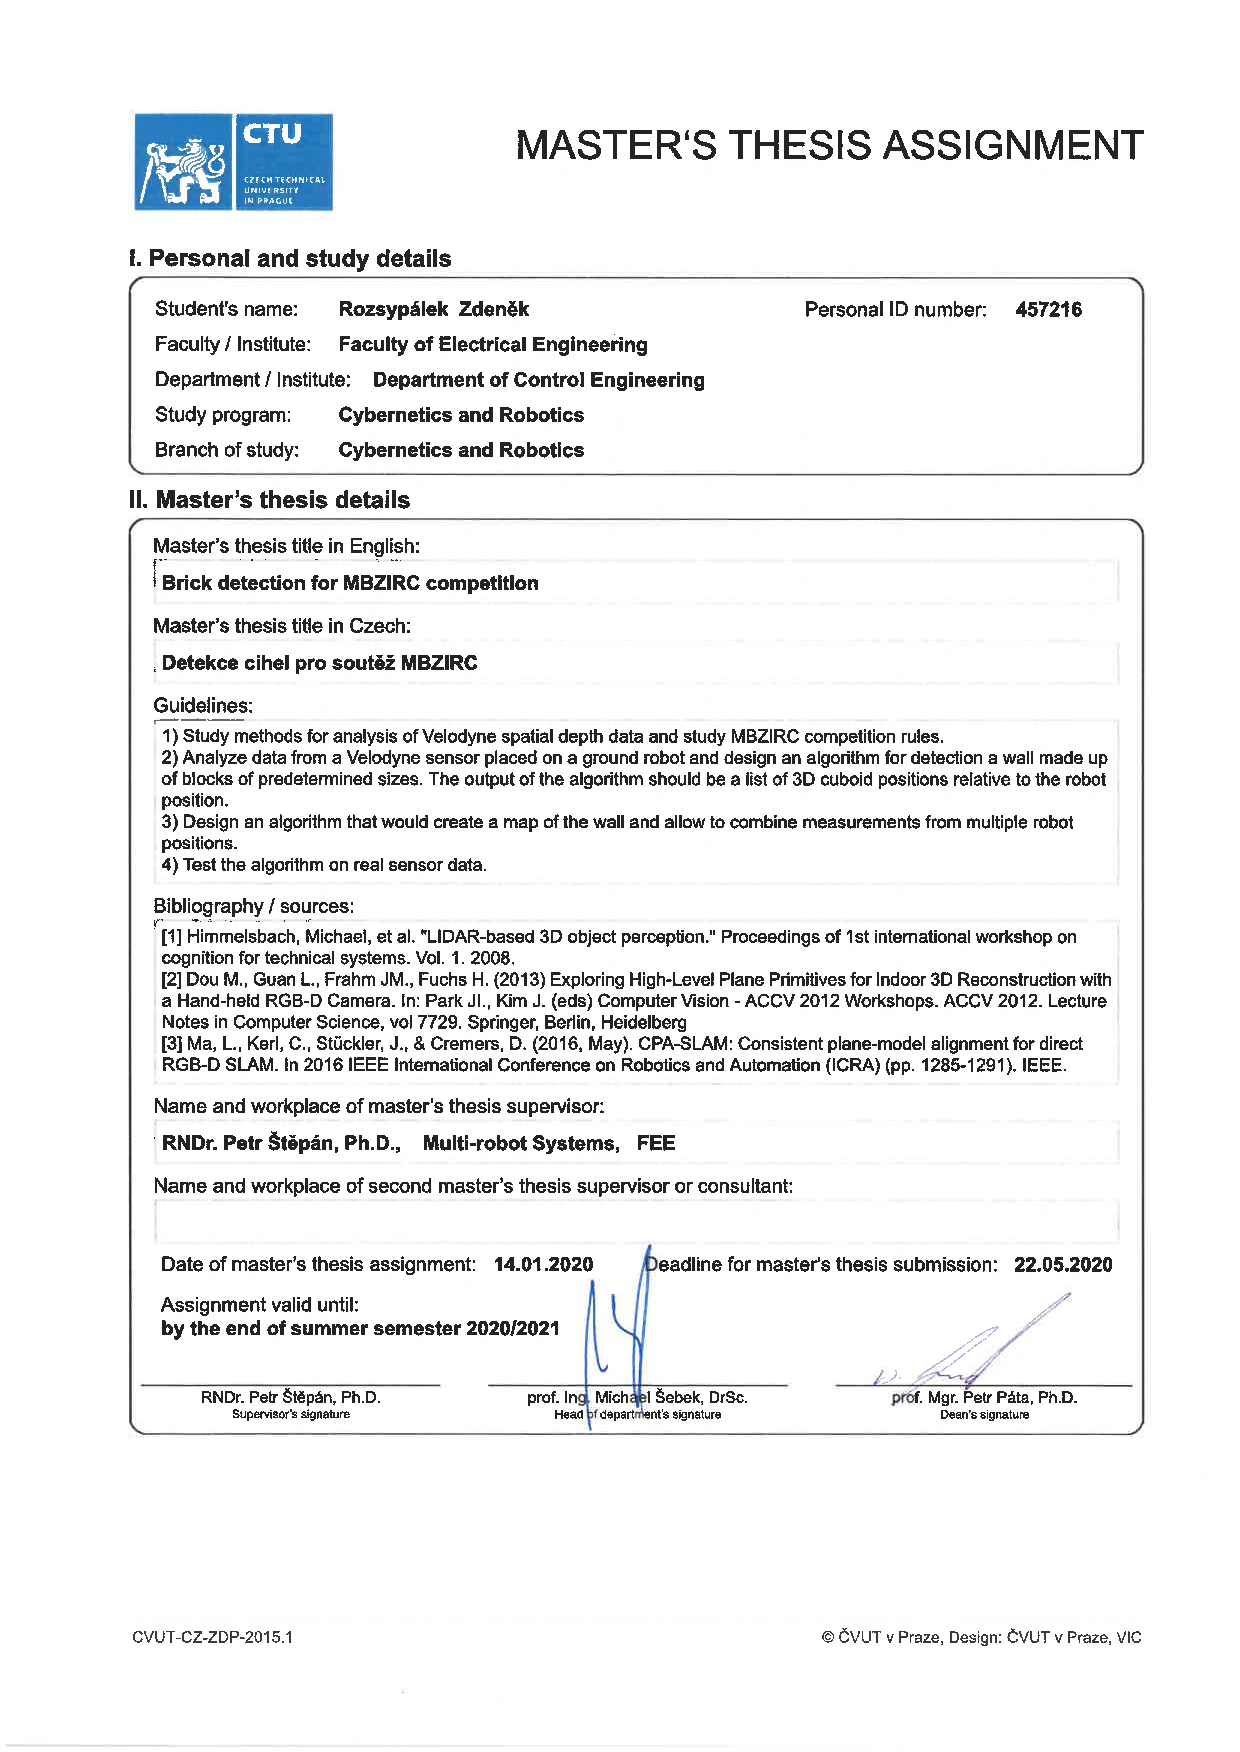
\includepdf[pages={1}]{zav_prace.pdf}
\cleardoublepage

~\vfill{}

\section*{Acknowledgements}

I would like to express my appreciation to Ing. Tomáš Petříček for his valuable and constructive suggestions during the planning and development of this thesis. I would also like to thank to the Department of Cybernetics of the Czech Technical University and to Michal Němec for the provided hardware. Finally, I wish to thank my family for support throughout my study.

\vspace{2.5cm}

\newpage{}

\cleardoublepage % it is prefered for the 1. level sections to start on the 

\vfill
\begin{center}
{\it \large Abstract}
\vspace{0.2cm}

\begin{minipage}{0.8\textwidth}{
The MBZIRC contests are focused on using autonomous multi-robot systems for tasks that are motivated by real-world problems. One of the tasks was to exploit the group of drones and ground robots to build a wall from bricks. Because all robots have to operate autonomously, it is crucial to have a system that can reliably detect the bricks. The set of methods that were used to detect these bricks is described in the thesis. Most of the methods are based on the lidar data measured by the ground robot. The lidar scans are processed by the split and merge algorithm to find the bricks in a very sparse pointcloud. Further, the RANSAC algorithm is applied from close range to verify the spatial distribution of different types of bricks. Moreover, the maximum likelihood estimate of the brick pile model, for usage in the EM algorithm, is derived. With a proper model and symbolic map, it is possible to poll previously saved partial measurements with different levels of confidence and obtain a position of any large spatially distributed object.
\vspace{3mm}
\par \textbf{Keywords:} MBZIRC, object detection, lidar, pointcloud, hypothesis fitting, EM algorithm, RANSAC
}
\end{minipage}
\end{center}
\vfill
\vspace{1cm}

\vfill
\begin{center}
{\it \large Abstrakt}
\vspace{0.2cm}

\begin{minipage}{0.8\textwidth}{
Soutěž Mohamed Bin Zayed International Robotic Challenge (MBZIRC) se zaměřuje na použití autonomních multi-robotických systémů pro úkoly, které jsou motivovány problémy reaálného světa. Jedním z úkolů bylo využít skupinu dronů a pozemní roboty pro postavení zdi z cihel. Jelikož všichni roboti museli pracovat plně autonomně, bylo naprosto nezbytné navrhnout systém, který může cihly spolihlivě detekovat. Diplomová práce popisuje metody, které byly použity pro detekci těchto cihel. Většina metod je založena na zpracování dat z lidaru, který nese pozemní robot. Paprsky z lidaru jsou zpracovány algoritmem split and merge, což umožňuje nalézt pozice cihel ve velmi řídkém mraku bodů. Dále je použit algoritmus RANSAC, který z malé vzdálennosti může ověřit vzájemné pozice různých druhů cihel. Kromě toho byl udělán odhad maximální věrohodnosti pro model hromady cihel, který je využit v inovativní aplikaci EM algoritmu. Pokud je použit správný model je takto možné nalézt jakýkoliv velký prostorově rozložený objekt pouze na základě částečných měření, s rozdílnou úrovní jistoty, uložených do symbolické mapy.
}
\end{minipage}
\end{center}
\vfill
\vspace{1cm}
\newpage{}

\cleardoublepage

\pagenumbering{roman}
\cfoot{\thepage}

\tableofcontents
\cleardoublepage

\listoffigures
\cleardoublepage


\pagestyle{fancy}
\fancyhf{}
\pagenumbering{arabic}
\cfoot{}
\fancyfoot[RO,RE]{\thepage$/$\pageref{LastPage}}
\setlength{\parskip}{0.35cm}

\fancyhead[LO,LE]{INTRODUCTION}
\chapter{Introduction}
\label{ch:intro}
Autonomous robotics experienced rapid development in the last decades. There are broad ranges of applications from heavy work in the industry to autonomous cars or space exploration. The two latter mentioned applications are very challenging, mainly because they require many abilities that are specific to the area of mobile robotics. Unlike in industry where robots usually perform repetitive tasks in an unchanging environment, the mobile robot must be aware of its surroundings. The robot is usually equipped with various sensors that provide information about the environment to enable the robot to perform complex tasks. Machine perception is a subfield of autonomous robotics which is dedicated to interpreting these sensors' output data.

The thesis is focused mainly on processing the data from a lidar (Light Detection And Ranging) sensor. The lidar is a laser-based rangefinder that uses the passive reflection of a detected object. It has a wide spectrum of usage, and it is also very popular in autonomous robotics. These applications are frequently using a spinning version of the lidar, which can cover $360\degree$ around the robot. In recent years companies like Ouster or Velodyne significantly reduced the cost and improved the quality of this technology, which led to further increasing interest. The classical applications includes collision avoidance \cite{sabatini2007}, SLAM \cite{kohlbrecher2017} or detection \cite{himmelsbach2008}.

The goal of this thesis is to present a detection algorithm for the MBZIRC 2020 (Mohammed Bin Zayed International robotic challenge). The contest aims at the development of autonomous robotics and presents challenging problems that must be resolved before the robots can be applied in the real world. All of the participants are further motivated by the prize money for the winner.

Chapter \ref{ch:intro} presents a problem, used equipment and software. The state-of-the-art methods are also discussed. In Chapter \ref{ch:methods} are proposed general methods that can be used for solving the problem. In Chapter \ref{ch:applications} are introduced tweaks to previously presented methods, which are necessary for our use-case. Chapter \ref{ch:experiment} contains a description of the conducted experiment and performance analysis of all methods. Last Chapter \ref{ch:conclusion} is devoted to the evaluation and conclusion.

\section{State of the art}
Because lidar is the most precise depth measuring sensor, it is often used for object detection in 3D space. Many proposed detectors use various machine learning methods. The SVM method was successfully used for classification before the boom of neural networks \cite{himmelsbach2008}. Nowadays, the most popular solutions are the ones powered by deep neural networks. CNNs (Convolutional Neural Networks), which operate on a 3D voxel map, are often used \cite{zhou2017}. This Voxel network architecture provides an end-to-end solution and can detect and classify on voxel map in one run. Many other architectures, which can improve the performance of such a network, were proposed. For example, slightly different CNN architectures or loss functions \cite{yan2018}. 

These networks have excellent performance, but they are developed mainly for use in autonomous vehicles. That means that they are trained on large annotated datasets, and they are usually computationally intensive (they require GPU). Moreover, the networks are used on quite a dense voxel map, which is generated by lidar with very high vertical resolution. Well known KITTI dataset was captured by lidar with more than four times higher vertical resolution than the lidar used in this thesis \cite{geiger2013}.

Very unpleasant is that the brick is very often hit by only one lidar layer. That is caused by the small size of the brick and low resolution of the lidar. We concluded that using some advanced feature extractor is unnecessarily complex to detect objects which manifest in lidar data as a simple line. Furthermore, these classifiers usually require large annotated datasets that are not available for our problem. Instead, we use more legacy approaches involving mainly line segmentation algorithms.

\section{MBZIRC Contest}
The contest took place in March in Abu Dhabi. The whole competition consisted of three challenges and the grand challenge, which connected all challenges. The first challenge was the only one that was focused solely on UAVs (unmanned aerial vehicles). The goal of the first challenge was to pop multiple big-colored balloons and catch a small ball carried by the organizer's drone. The other two challenges were designed for both UGVs (unmanned ground vehicles) and UAVs. 

The second challenge was about building a wall using robots. Multiple polystyrene bricks were placed in the arena, and the robots should have moved these bricks to the destination area and stack them on top of each other to build the wall. 

The third challenge was to extinguish a fire on the surface of the building model. This task was motivated by the inability of firefighters to extinguish fire inside high-rise buildings in United Arab Emirates. UAVs and UGVs carried tanks full of water and squirted it into the fire dummy. Every team had three rehearsals before the contest, and then two competition attempts for each one of the three challenges. Only the best teams from all three challenges were nominated into the grand challenge, which was limited to just one attempt.

\subsection{Second Challenge}
This thesis is focused on the second challenge, specifically on the ground robot section of the second challenge, so that we provide a more detailed description. Each team is given thirty minutes to explore the arena ($40$m$\times 60$m), localize all interest areas, and build the wall. There are four types of bricks with different colors. All bricks must be very light to enable the UAVs to pick them up. The dimension and colors of the bricks can be seen in Figure \ref{fig:brickdef}. The team obtains points for every placed brick. Bricks with different colors are rewarded by a different number of points. Placing bigger bricks means higher rewards. In addition, the UAV bricks are rewarded by twice as many points as the UGV bricks.

\begin{figure}[H]

\centering
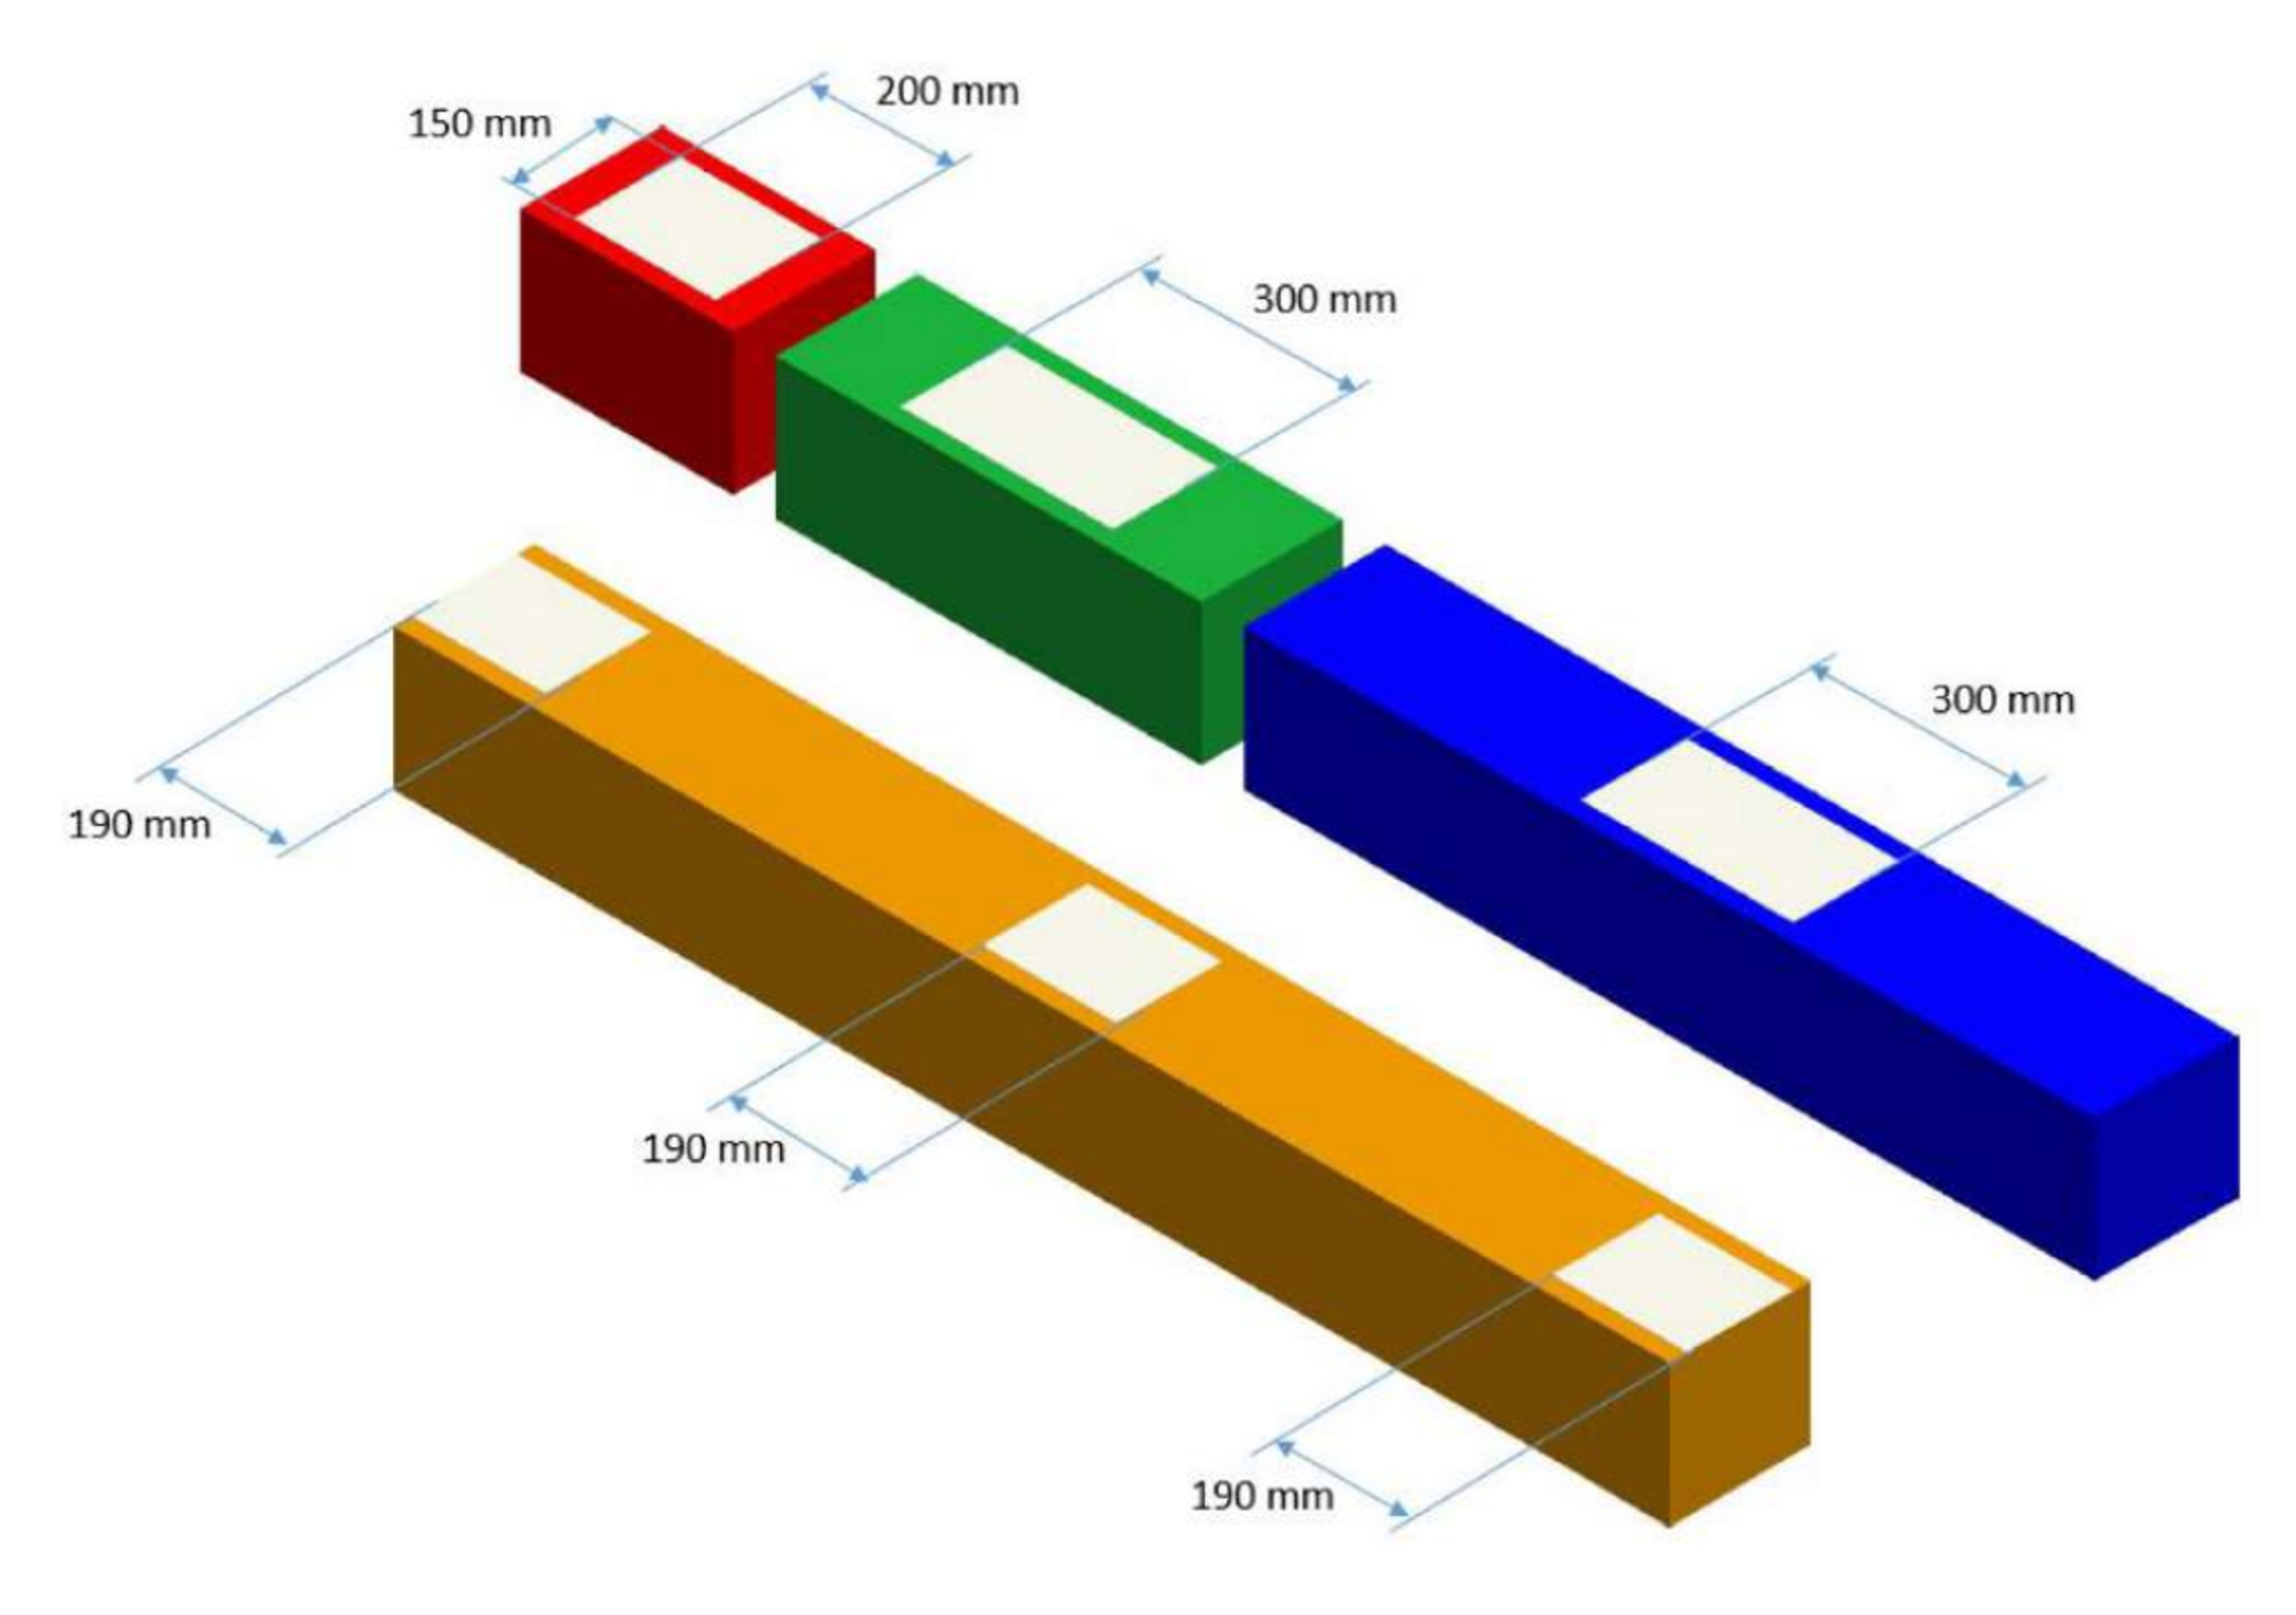
\includegraphics[scale=0.33]{fig/brick_sample.png}
\caption[Bricks definition]{Colors and dimensions of the bricks provided by the organizer.}
\label{fig:brickdef}

\end{figure}

Each brick has a thin metal plate on top of it so that the robots are able to pick them up using electromagnets. At the beginning of the challenge, all bricks are placed in a beforehand unknown position. The initial position of bricks is unknown, but there is a predefined pattern in which the bricks are put together. There are different patterns for the UGV piles of bricks and the UAV piles. The UGV bricks are stacked into the multiple height levels, whereas the UAV bricks are stacked into the width, and all are put on the ground. Due to the low weight of the bricks, it is necessary to put UAV bricks into the rails. Otherwise, the bricks could be easily blown away by the propellers of the drones. Since the UAV bricks are all on the ground level (in the purely horizontal pattern), detecting them with the UAV bottom camera is much easier than using the lidar. That is why we are further concerned only about UGV bricks. These bricks are stacked in the positions displayed in Figure \ref{fig:piledef}.

\begin{figure}[H]

\centering
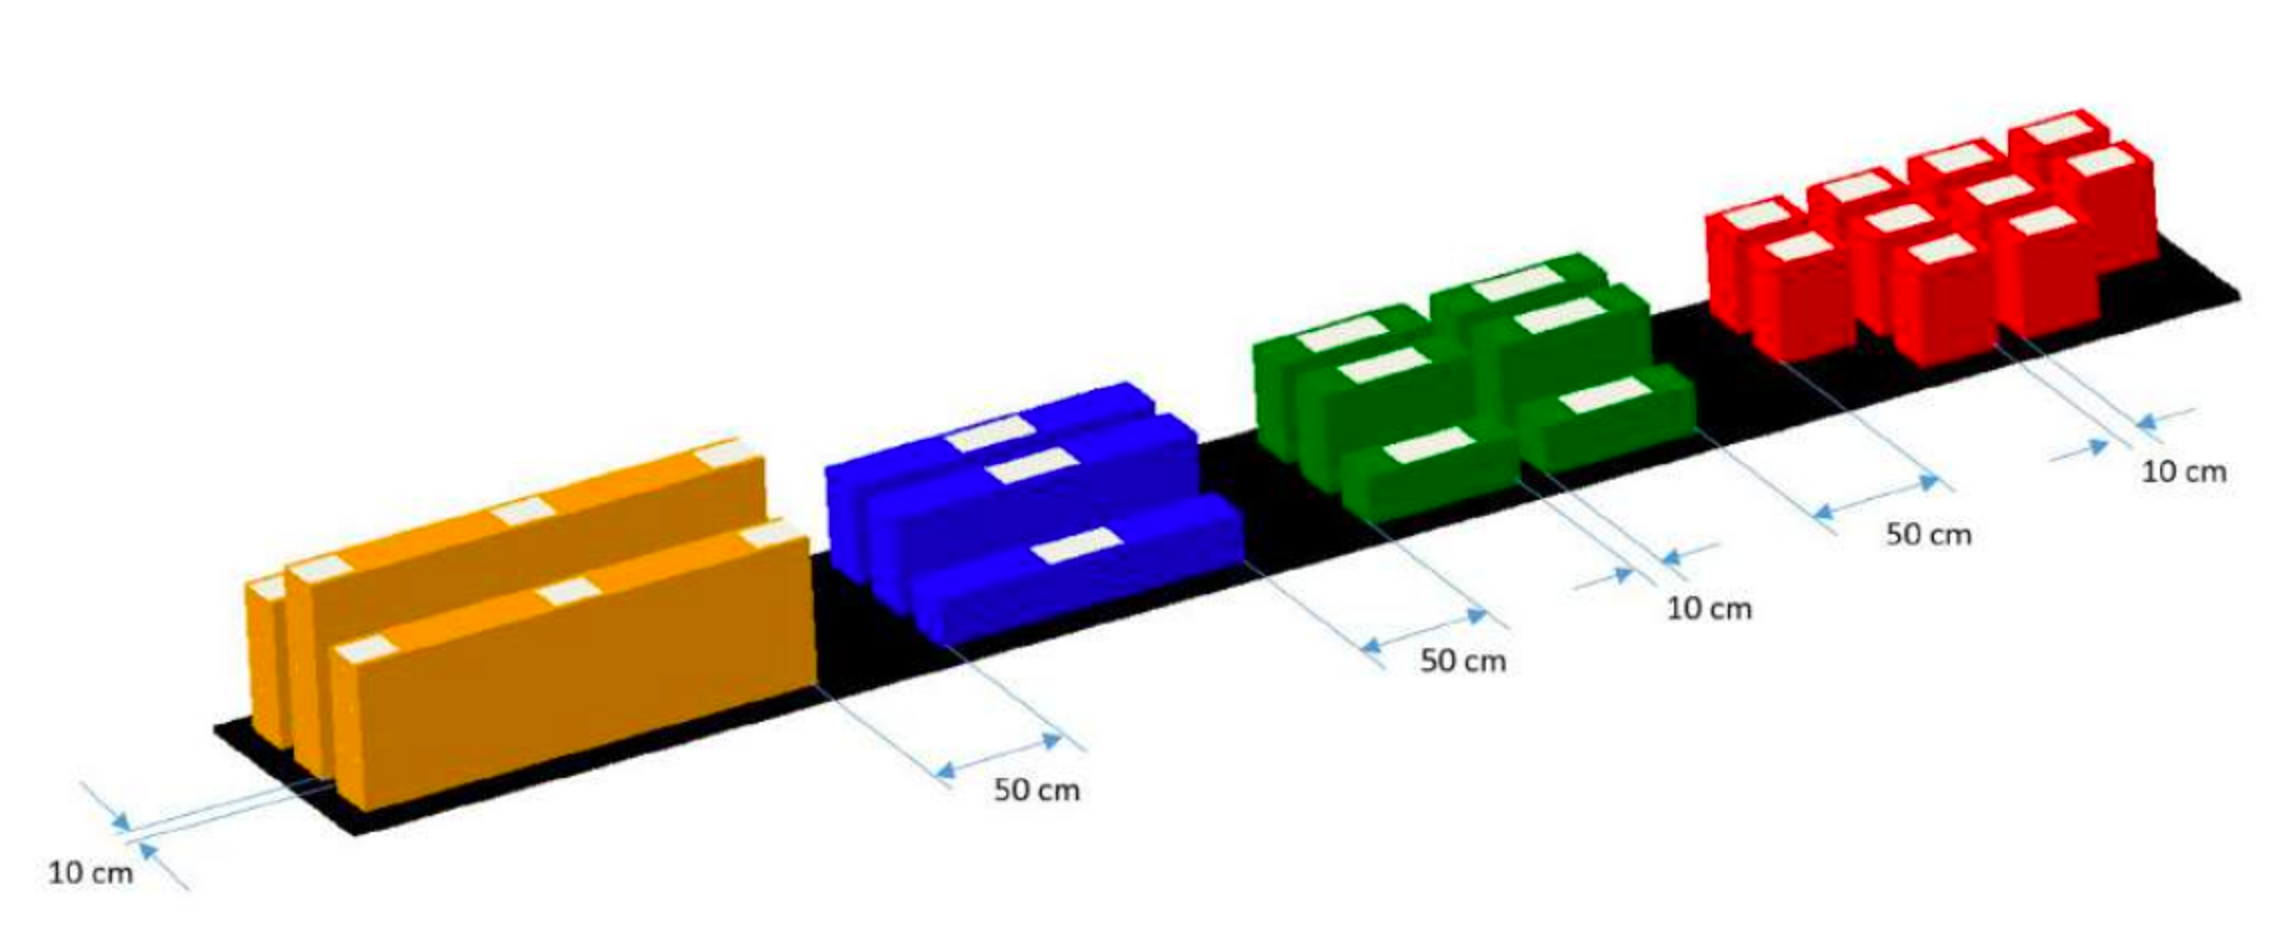
\includegraphics[scale=0.35]{fig/initial_layout.png}
\caption[Initial brick layout]{The positions of the bricks at the beginning of the second challenge.}
\label{fig:piledef}

\end{figure}

Other objects of interest are destinations where the bricks should be placed. The robots must look for them during the exploration. UGV brick's destination is marked by a checker pattern. Detecting the pattern was very challenging because the exact shape was not known until the second rehearsal. The final form of the pattern is shown in Figure \ref{fig:checker}. Although we are not concerned about the UAV bricks, the destination of the UAV bricks is a vertical object, so it is much easier to detect it from the ground using the lidar. The UAV bricks destination is a wall, as seen in Figure \ref{fig:uavdest}. Bricks should be placed on top of this wall. The metal plate on top of each brick shifts the center of mass to the top and make the brick very susceptible to rolling. That is why are the auxiliary handles mounted on the top of the UAV destination wall. At the beginning of the challenge, each team is given the instructions which describe how the wall should look like at the end. When the built wall does not fit the instructions, the team gets a penalty and gains fewer points for inaccurately placed bricks.


\begin{figure}[H]
\centering
\begin{subfigure}{.3\textwidth}
  \centering
\vspace{18mm}

\includegraphics[scale=0.1]{fig/pattern.pdf}
\vspace{18mm}
\caption[UGV destination]{UGV destination pattern.}
\label{fig:checker}
\end{subfigure}
\begin{subfigure}{.65\textwidth}
  \centering
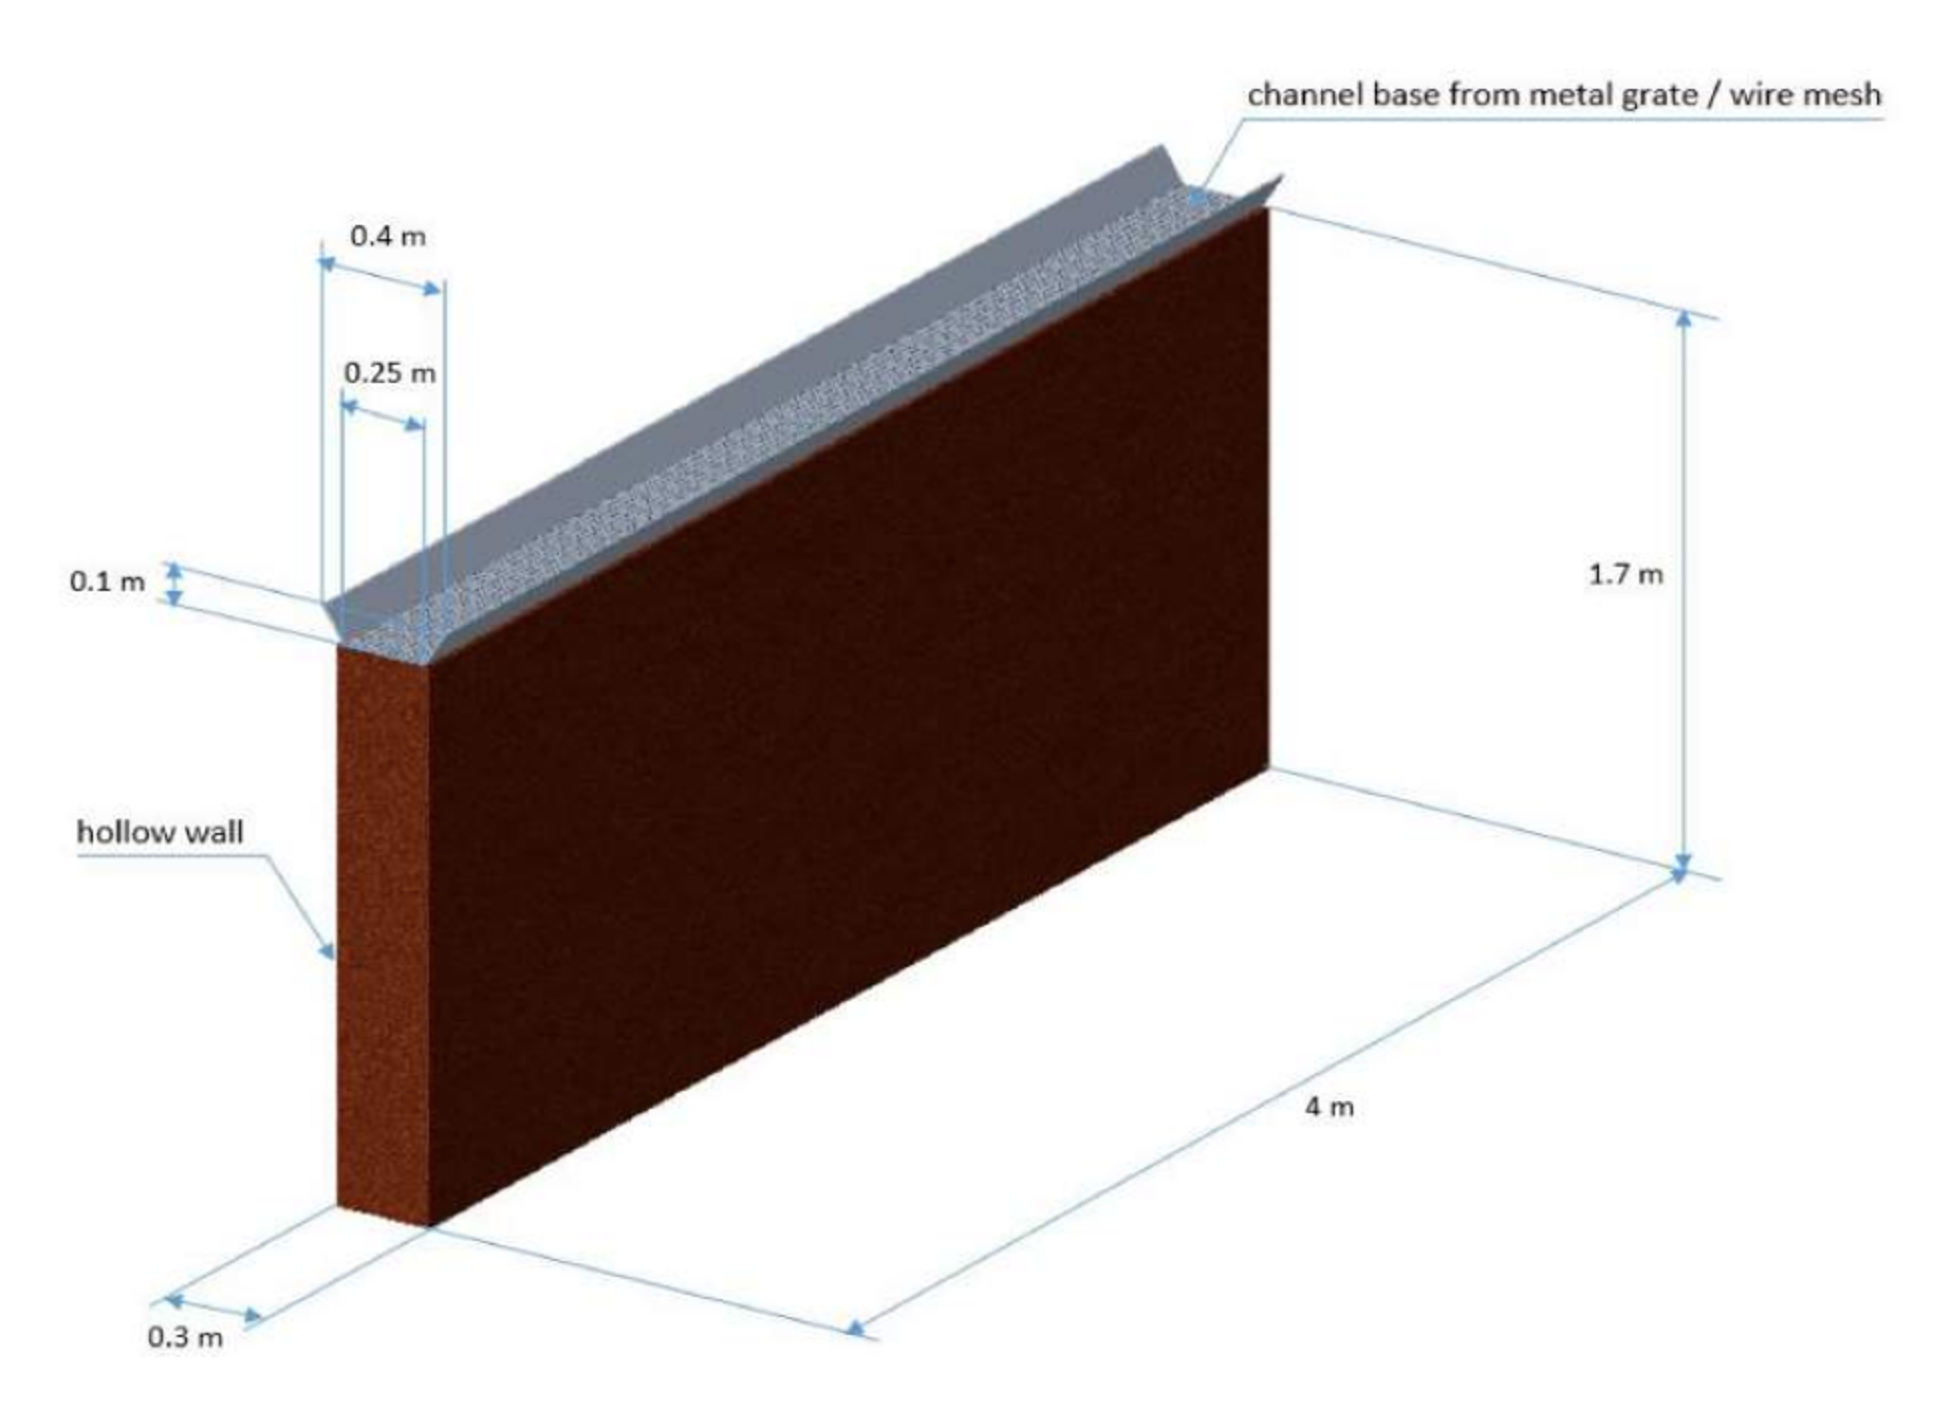
\includegraphics[scale=0.35]{fig/wall_sample.png}
\caption[UAV destination]{UAV destination}
\label{fig:uavdest}
\end{subfigure}

\caption[Brick destinations]{Description of target places for UAVs and UGVs. Each square in the UGV pattern has a width of $0.1$m. The pattern consists of two $4\times0.4$m segments, which are connected into the \textit{L} shape. Whole UAV destination consists of four similar segments arranged into the \textit{W} shape with right angles.}
\label{fig:dest}
\end{figure}


\section{Equipment}
For the sake of completeness, it is necessary to describe what exact equipment was available. We used \textbf{Clearpath Husky A200}, which is a wheeled robot designed for outside robotics. The robot was equipped with many additional devices. \textbf{Intel NUC} was used as a computer to run the code and control the robot. The \textbf{Kinova robotic arm} was mounted on top of the Husky robot to manipulate the bricks. Two \textbf{12V electromagnets} were attached to the end-effector to enable the arm to grip the bricks. It would be tough to grip the bricks without any feedback loop to the hand. For visual servoing and proper gripping, we placed \textbf{Intel Realsense} camera close to the end of the arm. It is also possible to obtain feedback from electromagnets thanks to hall effect sensors and decide whether the brick is gripped correctly. For the localization, collision avoidance and detection was used \textbf{Velodyne VLP-16} lidar sensor. Lastly, to move the bricks around the arena, we created a handmade cargo area that can contain up to six bricks and attached it to the rear bumper. It was not possible to carry more bricks mainly because of restrictions on the robot's size and also due to the limited range of Kinova arm. The whole setup is captured in Figure \ref{fig:husky}.

\begin{figure}[H]
\centering
\includegraphics[scale=0.275]{fig/husky.png}
\caption[UGV robot setup]{Clearpath Husky A200 adjusted for the second challenge.}
\label{fig:husky}

\end{figure}

\subsection{Velodyne VLP-16}
This thesis deals mainly with lidar data. Therefore, the following subsection provides a more detailed description of the lidar sensor. Inside the VLP-16 puck, there is a rotating infrared laser of class one, which measures the distance using the time of flight principle. A 12V power supply powers lidar and the data are transferred via UDP packets over the ethernet. The configuration of the Velodyne lidar used for the contest is described in Table \ref{tab:lidar}. The lidar can be set up with a slightly better resolution, but there is a trade-off between resolution and frequency, and we preferred higher frequency over the resolution.

\begin{table}[H]
\centering
\caption{Parameters of the VLP-16 lidar sensor.}
\begin{tabular}{lr}
\toprule
Parameter & Value \\
\midrule
Layers [-]                            & 16   \\ 
Maximal Range [m]                         & 100  \\
Vertical FOV [$\degree$]          & $\pm15$   \\ 
Vertical resolution [$\degree$]   & 2    \\ 
Horizontal FOV [$\degree$]        & 360  \\ 
Horizontal resolution [$\degree$] & 0.4  \\ 
Frequency [Hz]                    & 20    \\ 
Precision [m]                     & $\pm0.03$ \\ 
\bottomrule
\end{tabular}
\label{tab:lidar}
\end{table}

\section{Software}
The operating system which is installed on the Intel NUC hard drive is Ubuntu 18.04. All necessary subroutines for controlling the robot are run by the Robot Operating System (ROS) \cite{ros}. That is a flexible framework for operating various robots or multi-robot systems. It offers many different tools and packages which can vastly simplify development, debugging, and deploying of any robotic platform. ROS is written in C++, but offers bindings to other modern languages such as Python or Ruby. Our work is implemented in C++ because it achieves the best performance in terms of execution time, and it has the best community support. ROS precisely defines how the files must be structured within the package. ROS also offers a high encapsulation level where each executable is run as a node that can communicate with other nodes using the predefined protocols. The protocols are defined in the form of ROS messages, which are used in two different ways. One possibility is to transmit the data via the ROS topics. Topics represent the classical producer-consumer scheme, where multiple listeners can be joined to a single topic, whereas the publisher doesn't receive anything. The other possibility is a so-called service server that returns something on each request. The most important node is the ROS core, which runs the ROS master and the parameter server. ROS also provides advanced logging and package \textit{rosbag}, which can record any specified topic and save it for replay.

It is vital to know the precise location of the robot inside the arena. For localization, the robot uses a probabilistic Monte Carlo method, which is sometimes called the particle filtering. This algorithm fuses data from range finder and odometry and creates multiple hypotheses (particles) of the robot's position and rotation. Each hypothesis’s quality is evaluated by approximating posterior probability within a standard Bayesian formulation of the localization problem \cite{dellaert1999} \cite{thrun2000}. Firstly, it is necessary to create a map when the robot is placed in a new environment. There is a ROS package called Gmapping, which can simultaneously create the map and navigate the robot using the particle filter. When the map is created, it is not further necessary to run the Gmapping node because only the localization is needed. For the Monte Carlo localization on a predefined map, the ROS package called AMCL is used.

\cleardoublepage

\fancyhead[LO,LE]{METHODS}
\chapter{Methods}
In this section of the thesis are described methods that can be applied to the detection of the bricks. Only a brief description is provided, and all methods are presented in a general form.

\section{Lidar detection range analysis}
It is useful to know a possible range of detection based on the lidar sensor. This range influences how the robot explores the arena and influences the choice of used methods. Higher the detection range is, a lower number of waypoints is necessary to explore the whole arena. There is a limited time for exploration because brick pickup and brick placement take much time. The speed of pickup and placement is limited mainly by the speed of the Kinova arm. We estimate the maximal range using the Figure \ref{fig:range}.

\begin{figure}[H]
	\centering
	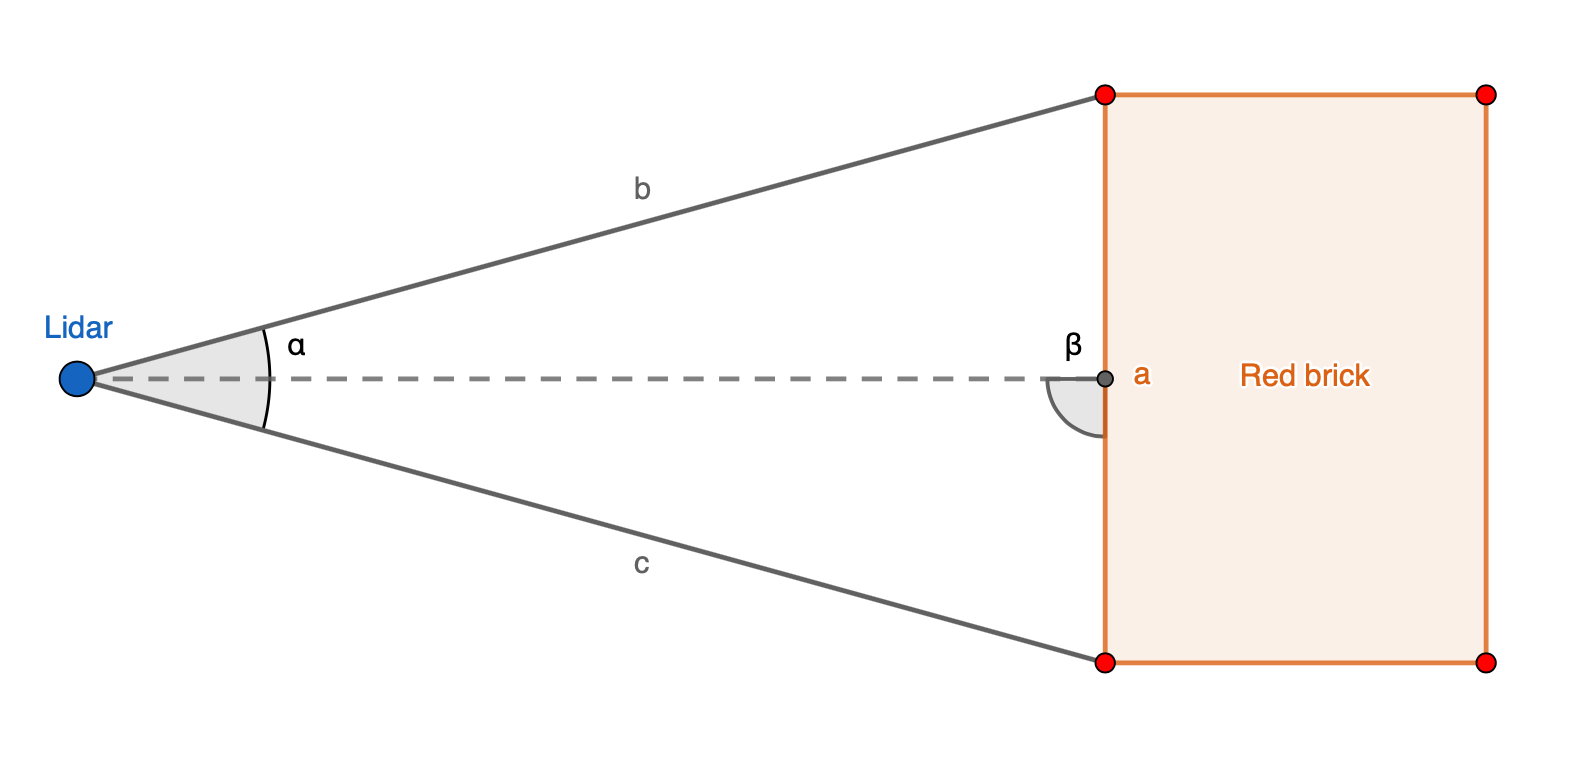
\includegraphics[scale=1.1]{fig/lidar_range.png}
	\caption[Lidar range study]{Visualization of rays hitting the red brick.}
	\label{fig:range}
\end{figure}

Angle $\alpha$ is the resolution of lidar known from table \ref{tab:lidar}. Only the maximal range is calculated, thus angle $\beta = 90\degree$. The cosine theorem can be used to obtain the distance between points on the brick.
\begin{equation}
a^2 = b^2 + c^2 - 2bc \cos \alpha.
\end{equation}
Because $\beta$ is right angle we can write $b = c$ and thus:
\begin{equation}
a = \sqrt{2b^2 \left(1-\cos \alpha \right)}.
\end{equation}
Now we want to know how many rays $N$ would hit the brick from given distance $b$ with lidar angular resolution $\alpha$ and the size of the brick $a$. 
\begin{align}
a &= \sqrt{2b^2 \left(1-\cos \left( N \alpha \right) \right)}, \\
N &= \frac{\arccos\left(1-\frac{a^2}{2b^2}\right) }{\alpha}.
\label{eq:rays}
\end{align}
Finally, we can plot a function of the number of rays $N$ with respect to distance to object $b$. This analysis can be done similarly for vertical and horizontal resolution.

\begin{figure}[H]
	\centering
	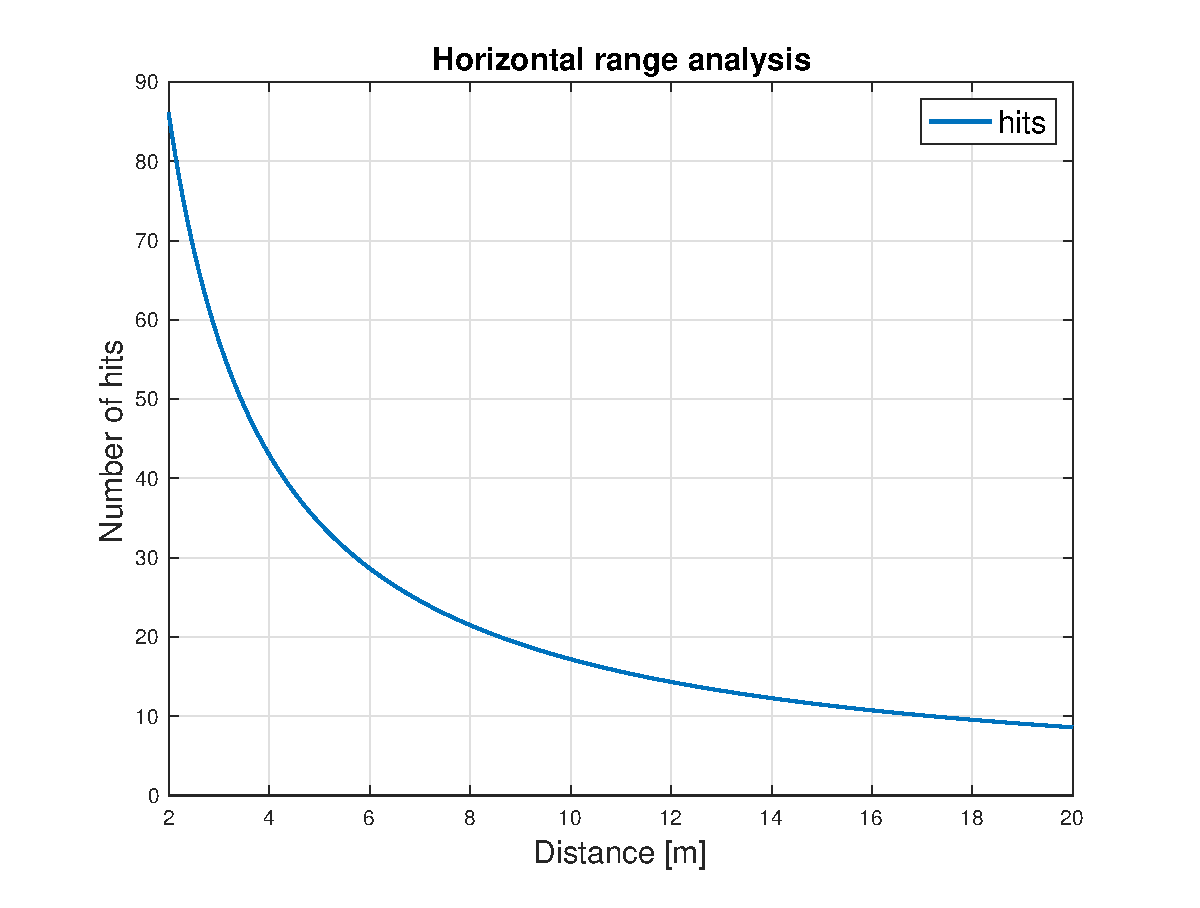
\includegraphics[scale=0.55]{fig/horizontal_range.eps}
	\caption[Horizontal range chart]{Number of hits of the smallest brick from given distance.}
	\label{fig:horizontal_hits}
\end{figure}

In Figure \ref{fig:horizontal_hits} is visible that the horizontal resolution of the lidar is not limiting factor of the range. Even from 10 meters is lidar able to hit red brick more than 15 times. On the other hand, the Figure \ref{fig:vertical_hits} shows that less than two lidar layers would hit the pile of bricks with a height of 40 cm from a distance greater than 6 meters. Furthermore, this is the best-case scenario analysis where $\beta$ is a right angle, which rarely happens in reality.

\begin{figure}[H]
	\centering
	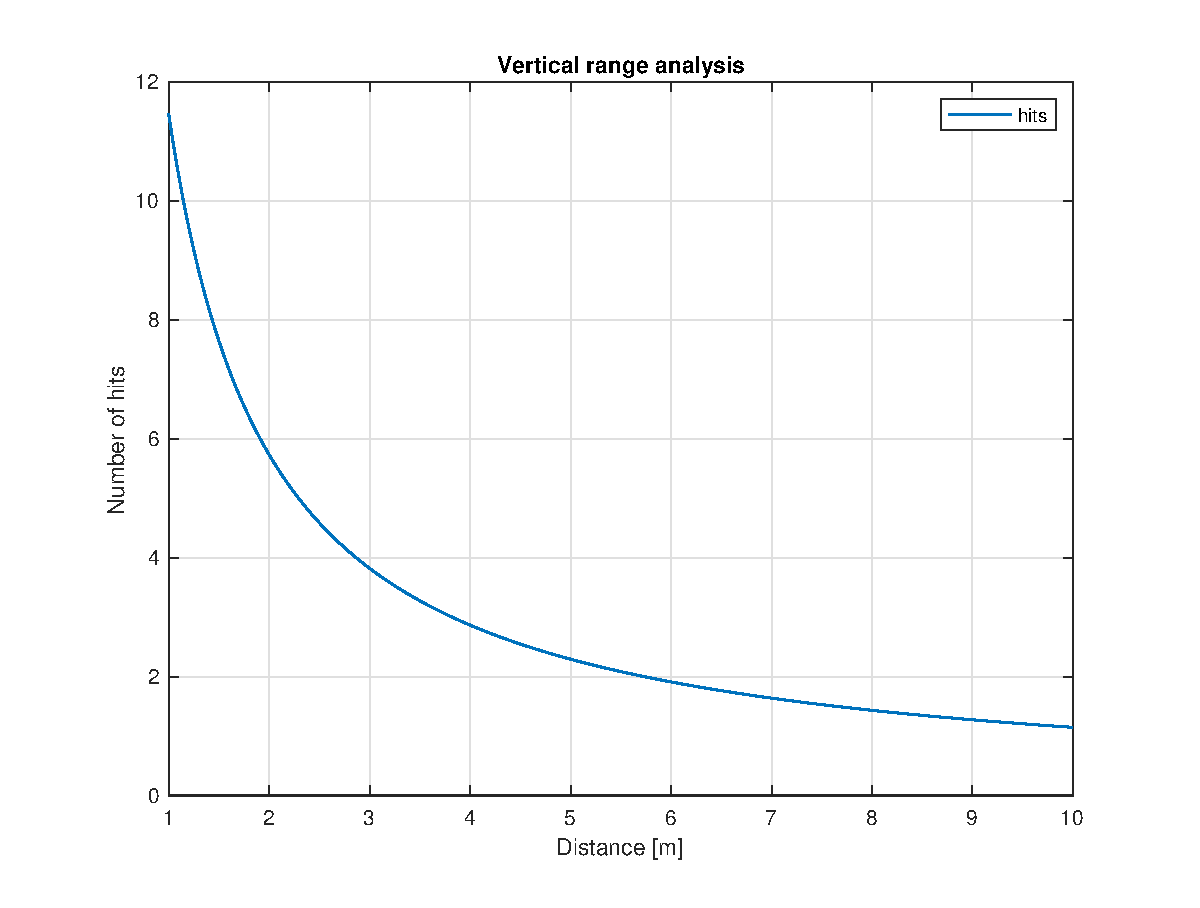
\includegraphics[scale=0.55]{fig/vertical_range.eps}
	\caption[Vertical range chart]{Number of hits of two stacked bricks from given distance.}
	\label{fig:vertical_hits}
\end{figure}

\section{Lidar data processing}

It would be handy to extract straight lines from lidar data to detect individual bricks. Several methods can be used to achieve this goal. One of the most popular algorithms for line extraction is currently split and merge algorithm. Initially was this algorithm proposed for image segmentation by Horowitz and Pavlidis \cite{horowitz1974}. A simple version of this algorithm for point-cloud processing is described in algorithm \ref{alg:segmentation}, where \textbf{C} is clustering distance and \textbf{S} is splitting distance. There are many implementations of this algorithm which differ mainly in a way how they compute some particular steps of the algorithm. For example, just the method of fitting a line to the cluster can vary a lot. The method of least squares is often used, but as a simple method as connecting endpoints of the cluster could be used. When the latter method is applied, the algorithm is usually referred to as Iterative End Point Fit (IEPF) \cite{siadat1997}. For the cluster creation, the points are iterated in each layer one by one. When the distance of the following points is too high, we split the cluster. Every cluster is then further recursively split based on the most distant point from the fitted line. In comparison to other line extraction algorithms is the split and merge algorithm, one of the best performings in terms of precision and computational complexity \cite{nguyen2006}.
\begin{algorithm}[]
 \KwData{pointcloud}
 \KwResult{line\_segments}
initialize constants C, S\;
  clusters = find\_clusters(pointcloud, C)\;
\While{clusters is not empty}{
	cluster = clusters.pop()\;
	line = fit\_line(cluster)\;
	point = most\_distant\_point(cluster, line)\;
	\eIf{distance(point, line) $>$ S}{
	   c1, c2 = split\_cluster(cluster, point)\;
		clusters.push\_back(c1, c2)\;
	}{
		line\_segments.push\_back(cluster[start], cluster[end])\;	
	}
}
merge\_parallel(line\_segments)\;
 
 \caption{Lidar data segmentation using split and merge algorithm.}
 \label{alg:segmentation}
\end{algorithm}


\section{EM algorithm}
Expectation-maximization (EM) algorithm is an iterative process that can find parameters of a specified statistical model based on incomplete data. One of the most used statistical description for the EM algorithm is the Gaussian mixture model. This model is particularly useful because it emerges in many real-world situations, and it is easy to maximize. As the name of the algorithm suggests, it repeats the expectation and maximization step. Each iteration of the algorithm should improve the likelihood of the model until the terminating criterion is met. The termination criterion can simply be the number of iterations, or the algorithm can be stopped when the model is not improving anymore. Although we are discussing mainly the Gaussian distribution, the EM algorithm can also be used for other distributions from exponential family \cite{dempster1977}. The usage of the EM algorithm for the classification of 3D lidar data is not an entirely novel approach. Gaussian mixtures were already used for terrain recognition \cite{lalonde2006}.
 
\subsection{Maximization}
For maximization step is used maximal likelihood estimate weighted by $\gamma$ from expectation step. For parameters of Gaussian distribution $\mathcal{N}(\mu, \sigma)$ and number of samples $N$ looks maximization as follows:
\begin{equation}
\mu = \sum_{n = 1}^{N} \gamma_n x_n, \\
\end{equation}
\begin{equation}
\sigma = \sum_{n = 1}^{N}\gamma_n (x_n - \mu)^2 .
\end{equation}

A critical assumption for the convergence of the algorithm is that its likelihood with respect to the estimated parameter must be concave. This can be easily proved by computing the second derivative of the likelihood function. For example, for the mean value of distribution  $\mu$, it is easy to show that the second derivative of likelihood is always negative, which means that the function has no local optima.
\begin{align}
\mathcal{L} &= \prod_{n=1}^N \mathcal{N}(x_n, \mu, \sigma), \\
\frac{\partial \log \mathcal{L}}{\partial \mu} &= \frac{1}{\sigma^2} \sum_{n = 1}^{N} (x_n - \mu), \\
\frac{\partial^2 \log \mathcal{L}}{\partial \mu^2} &= \frac{-N}{\sigma^2}.
\end{align}

\subsection{Expectation}
The expectation step is done simply by evaluating conditional probability of current parameters given the sample:
\begin{equation}
\gamma_n = P(\mu, \sigma | x_n),
\end{equation}
which is calculated using the Bayes theorem and the law of total probability:
\begin{align}
\gamma_n &= \dfrac{P(x_n | \mu, \sigma) P(\mu, \sigma)}{P(x_n)}, \\
\gamma_n &= \dfrac{P(x_n | \mu, \sigma) P(\mu, \sigma)}{\sum_{k = 1}^N P(x_k | \mu, \sigma) P(\mu, \sigma)}.
\end{align}
There is only one class so the priors can be evaluated $P(\mu, \sigma) = 1$ and the equation simplifies to final form:
\begin{equation}
\gamma_n = \dfrac{\mathcal{N}(x_n, \mu, \sigma) }{\sum_{k = 1}^N \mathcal{N}(x_k, \mu, \sigma) }.
\end{equation}

\subsection{Algorithm}
How to implement a generic version of the EM algorithm on sampled data is shown in algorithm \ref{alg:em}, where \textbf{x} is the observed data samples. All relevant calculations for Gaussian distribution are described in previous subsections. It is not clear where to start iterating. It is possible to start both with the expectation and with the maximization step, but both parts are dependent on the result of the other one. Here we start with the maximization step, so during the initialization, we set $\alpha_n = 1$. If some prior information about the model's parameters is available, they can be set during the initialization, and the algorithm can be started with the expectation step. This informed initialization can remarkably reduce the number of iterations and sometimes even an outcome of the algorithm.
\begin{algorithm}[]
 \KwData{x}
 \KwResult{parameters $\theta$}
 set all $\alpha_n$ = 1\;
\While{not stopping\_criterion}{
	$\theta$ = maximization(x, $\alpha$)\;
	$\alpha$ = expectation(x, $\theta$)\;
} 
 \caption{Pseudocode shows how to implement the EM algorithm.}
 \label{alg:em}
\end{algorithm}


\section{RANSAC}
Random sample consensus (RANSAC) is an iterative method which can estimate parameters of the hypothesis given the data. It was first presented by Fischler \cite{fischler1981} with application in scene and image analysis, but it can be used for fitting arbitrary hypothesis. The most significant advantage of this algorithm is its robustness to outliers. The major drawback of this method is its high time complexity when fitting hypotheses to noisy data with a large number of samples. The whole iterative process is described in the algorithm \ref{alg:ransac}, where \textbf{x} is the observed data, \textbf{C} is the maximized cost and $\bm{\theta}$ are the parameters of the hypothesis.
\begin{algorithm}[]
 \KwData{x}
 \KwResult{best parameters $\theta^*$}
 initialize $\theta, \theta^*, C, C^*$\;
\While{not stopping\_criterion}{
	samples = draw\_samples(x)\;
	$\theta$ = find\_parameters(samples)\;
	$C$ = compute\_cost(x, $\theta$)\;
	\If{$C > C^*$}{
		$C^* = C$\;
		$\theta^* = \theta$\;
	}
} 
 \caption{Pseudocode shows how to implement the RANSAC algorithm.}
 \label{alg:ransac}
\end{algorithm}

The number of drawn samples in \textbf{draw\_samples} must be equal or higher than the number of degrees of freedom of the hypothesis. After drawing the samples method, \textbf{find\_parameters} assigns the correspondences between sampled data and the hypothesis. The correspondences are used to obtain the parameters of the hypothesis. Then the algorithm is evaluating the quality of the hypothesis by applying the hypothesis to the whole dataset. This quality estimate can be done by an arbitrary cost function. A common practice is to define some metrics in our domain and use a threshold value to obtain the number of samples that fit the hypothesis. These samples are often referred to as inliers. Stopping criterion is usually met when the probability of sampling a better hypothesis is lower than a specified threshold. This section describes just the basic version of the algorithm. Many improvements to the RANSAC algorithm was proposed since 1981 \cite{chum2008}.

\subsection{Tentative Correspondences}
The tentative correspondences can help us to choose better samples from the data to generate a better hypothesis. It is necessary to define some function witch measure the similarity between data and hypothesis. The data which has a higher similarity to the hypothesis is then chosen with higher probability. It is also possible to completely ban correspondences with low similarity. Given the typical application in scene analysis, the similarity is usually computed by comparing keypoint descriptors.

\section{Global model and transformations}
One of the goals of this thesis is to develop a global model that can efficiently store and update the positions of interest points. This global model is in the map coordinate frame. The localization of the robot is essential for the precise global model. Every detection must be transformed from the coordinate frame of the sensor to the coordinate frame of the map. Transformation can be easily done using matrix multiplication:
\begin{equation}
\begin{bmatrix}
x^\prime \\
y^\prime \\
z^\prime 
\end{bmatrix}
=
R \begin{bmatrix}
x \\
y \\
z
\end{bmatrix}
+ \vec{t},
\end{equation}
where $R$ is $3\times3$ the rotation matrix and $t$ is a $1\times3$ translation vector between coordinate frames. Similarly the transformation can be done in homogenous coordinates by merging translation and rotation into one matrix $T$:
\begin{equation}
\begin{bmatrix}
\vec{x}^\prime \\
1
\end{bmatrix}
=
\begin{bmatrix}
 \bm{R} & \vec{t} \\
 \vec{0} &  1
\end{bmatrix}
\begin{bmatrix}
\vec{x}\\
1
\end{bmatrix}.
\end{equation}

Different framework for computing the transformations is using quaternions. The quaternions are currently the standard for transformations in computer graphics and robotics. The most significant advantage of quaternions is that they are more efficient and do not suffer from gymbal lock and ambiguity of rotation. Arbitrary rotation and scaling can be expressed as quadruple of numbers in the quaternion framework. The rotation between coordinate frames $B \to A$ is computed with quaternions as:
\begin{equation}
q_A = q_T q_B q_T^*,
\end{equation}
where $q_A$ is quaternion in coordinate frame $A$, $q_B$ is quaternion in coordinate frame $B$, $q_T$ is quaternion representing the transformation between these coordinate frames, and $q_T^*$ is its conjugate. There is available a library within the ROS which can handle all these transformations in different forms \cite{tf}. 

\subsection{Symbolic map}
When all detections are transformed into the map frame, we can add them to a symbolic map. The symbolic map is storing the positions of all interest points and makes up the global model of the arena. Every object added to the symbolic map has a float number, which indicates the confidence of detection. When there is a new detection within a specific range from an object already stored in the symbolic map, a new object is not added, but only the confidence is increased. This approach creates clusters of interest points of different types. All interest points can be polled from the symbolic map, and the robot can make decisions based on the confidence of such an interest point. The symbolic map also checks whether the inserted object is located inside the arena. Otherwise, the object is rejected. (CITACE)

\subsection{Lidar to camera registration}
As can be seen in Figure \ref{fig:brickdef} (where the bricks are defined) besides the dimensions, another important feature of the bricks is their color. Although the color manifests itself a little bit in reflectivity of the surface, which can be detected by lidar, it is not possible to reliably distinguish the colors using only the lidar sensor. Until there is a gap between the individual bricks, it is possible to detect brick using just the spatial data. Ideally, the robot should be stacking bricks next to each other without any significant gap. Without any information about the color, it is impossible to decide whether the robot is detecting one large brick or several small bricks put together. So for this part of detection is necessary to color the point-cloud. Coloring can be done by using the image from Intel RealSense camera and projecting a 3D lidar point-cloud to the camera plane. For this purpose is used the pinhole camera model. To describe such a model is used intrinsic camera matrix $K$ which consists of intrinsic camera parameters \cite{hartley2017}
\begin{equation}
K = \begin{bmatrix}
f_x & 0 & c_x \\
0 & f_y & c_y \\
0 & 0 & 1
\end{bmatrix},
\end{equation}
where $f_x, f_y$ are focal lengths and $c_x, c_y$ stands for optical center of the camera.

Firstly is necessary to transform the whole point-cloud from the lidar coordinate frame to the camera frame. For this purpose, so-called extrinsic camera parameters are used, which describe where a camera is placed in the lidar coordinate frame. This type of transformation is discussed at the beginning of this section. Secondly, we can use the intrinsic camera parameters to calculate the projection. Note that it is needed to work in a homogenous 2D coordinate system.
\begin{equation}
\begin{bmatrix}
u\\
v\\
1
\end{bmatrix}
= K \begin{bmatrix}
x\\
y\\
z
\end{bmatrix}.
\end{equation}
It is possible to decide which coordinates $u,v$ on image plane corresponds to 3D point $x,y,z$ from point-cloud, and assign the color of a specific pixel to the point, using this matrix equality. However, this works only for the simplest pinhole camera model without any distortion of the image. If the lens has non-negligible distortion, this distortion must be included in the camera model. For the description of distortion are used the distortion coefficients.

\newpage
\cleardoublepage

\fancyhead[LO,LE]{APPLICATION OF METHODS}
\chapter{Application of methods}
\label{ch:applications}
In the following part of the thesis is described how to apply discussed methods to our problem. It is necessary to make several adjustments and also combine some of these methods to ensure reliable detections.

\section{Detection pipeline}
Detection is divided into three parts. All three parts are discussed in the next three subsections. The detection pipeline is visualized in Figure \ref{fig:flowchart}. 

\hspace{5px}
\begin{figure}[H]
\centering
\includegraphics[scale=0.06]{fig/flowchart.pdf}
\caption[Program pipeline]{Visualization of detection pipeline.}
\label{fig:flowchart}
\end{figure}

It can be seen that the symbolic map has two types of inputs. The main advantage of this approach is that it extends the lidar detection range. As discussed in the previous section, the used lidar has a low vertical resolution of only 16 layers. Thus the bricks are often visible in only one layer of a lidar scan. If we use only one scan, there is a high probability of false-positive measurements. On the one hand, we can decrease the occurrence of false positives by adding other lidar layers into the detection process. But on the other hand, two layers are available only from a distance smaller than $6$m, and that decreases the detection range. Therefore we exploited both approaches. One layer line segmentation for generating the candidates with low confidence and multilayer pile detector providing high-quality estimates. 

It is essential to obtain positions in the map frame, but for grasping, it is also necessary to introduce an algorithm that can give real-time feedback to the robot frame to align itself with the brick pile. When the robot is too close to the pile, it is impossible to get feedback from lidar because the bricks can be occluded, or they can be closer than the minimal lidar range. Therefore the robot needs a camera servoing for fine alignment during the brick pickup.

\section{Line segmentation}
For line segmentation, the IEPF algorithm is used, which is very similar to the one described in Algorithm \ref{alg:segmentation}. Only the final merging of parallel segments is omitted because it can connect two bricks into one. After retrieving the segments, filtering based on the segment size is done. It is possible to assign the color to the segment because each brick type has a unique size. For this reason, a new constant $max\_err$ must be defined, which thresholds out detections of incorrect size. An example of lidar measurement with extracted and filtered lines is in Figure \ref{fig:segments}. 

Algorithm performance is influenced by the correct setup of constants $C$ and $S$ (clustering and splitting distance). If we choose C too high, the algorithm could join two bricks into one segment. As described in Figure \ref{fig:piledef}, the distance between two bricks of the same color is $0.1$m. Therefore the clustering distance must always be less than $0.1$m. If the clustering distance is too low, one brick can be unintentionally divided into many segments, and without merging at the end, these segments are useless. It is necessary to bear in mind that the lidar precision, as shown in Table \ref{tab:lidar} is $\pm0.03$m, so any clustering with a distance of similar magnitude would be highly affected by sensor noise. The found segments are transformed into the map frame and passed to the symbolic map as low confidence detections. The segments are further passed to the pile detector, which can filter out false-positive detections.

\hspace{8mm}

\begin{figure}[H]
\centering
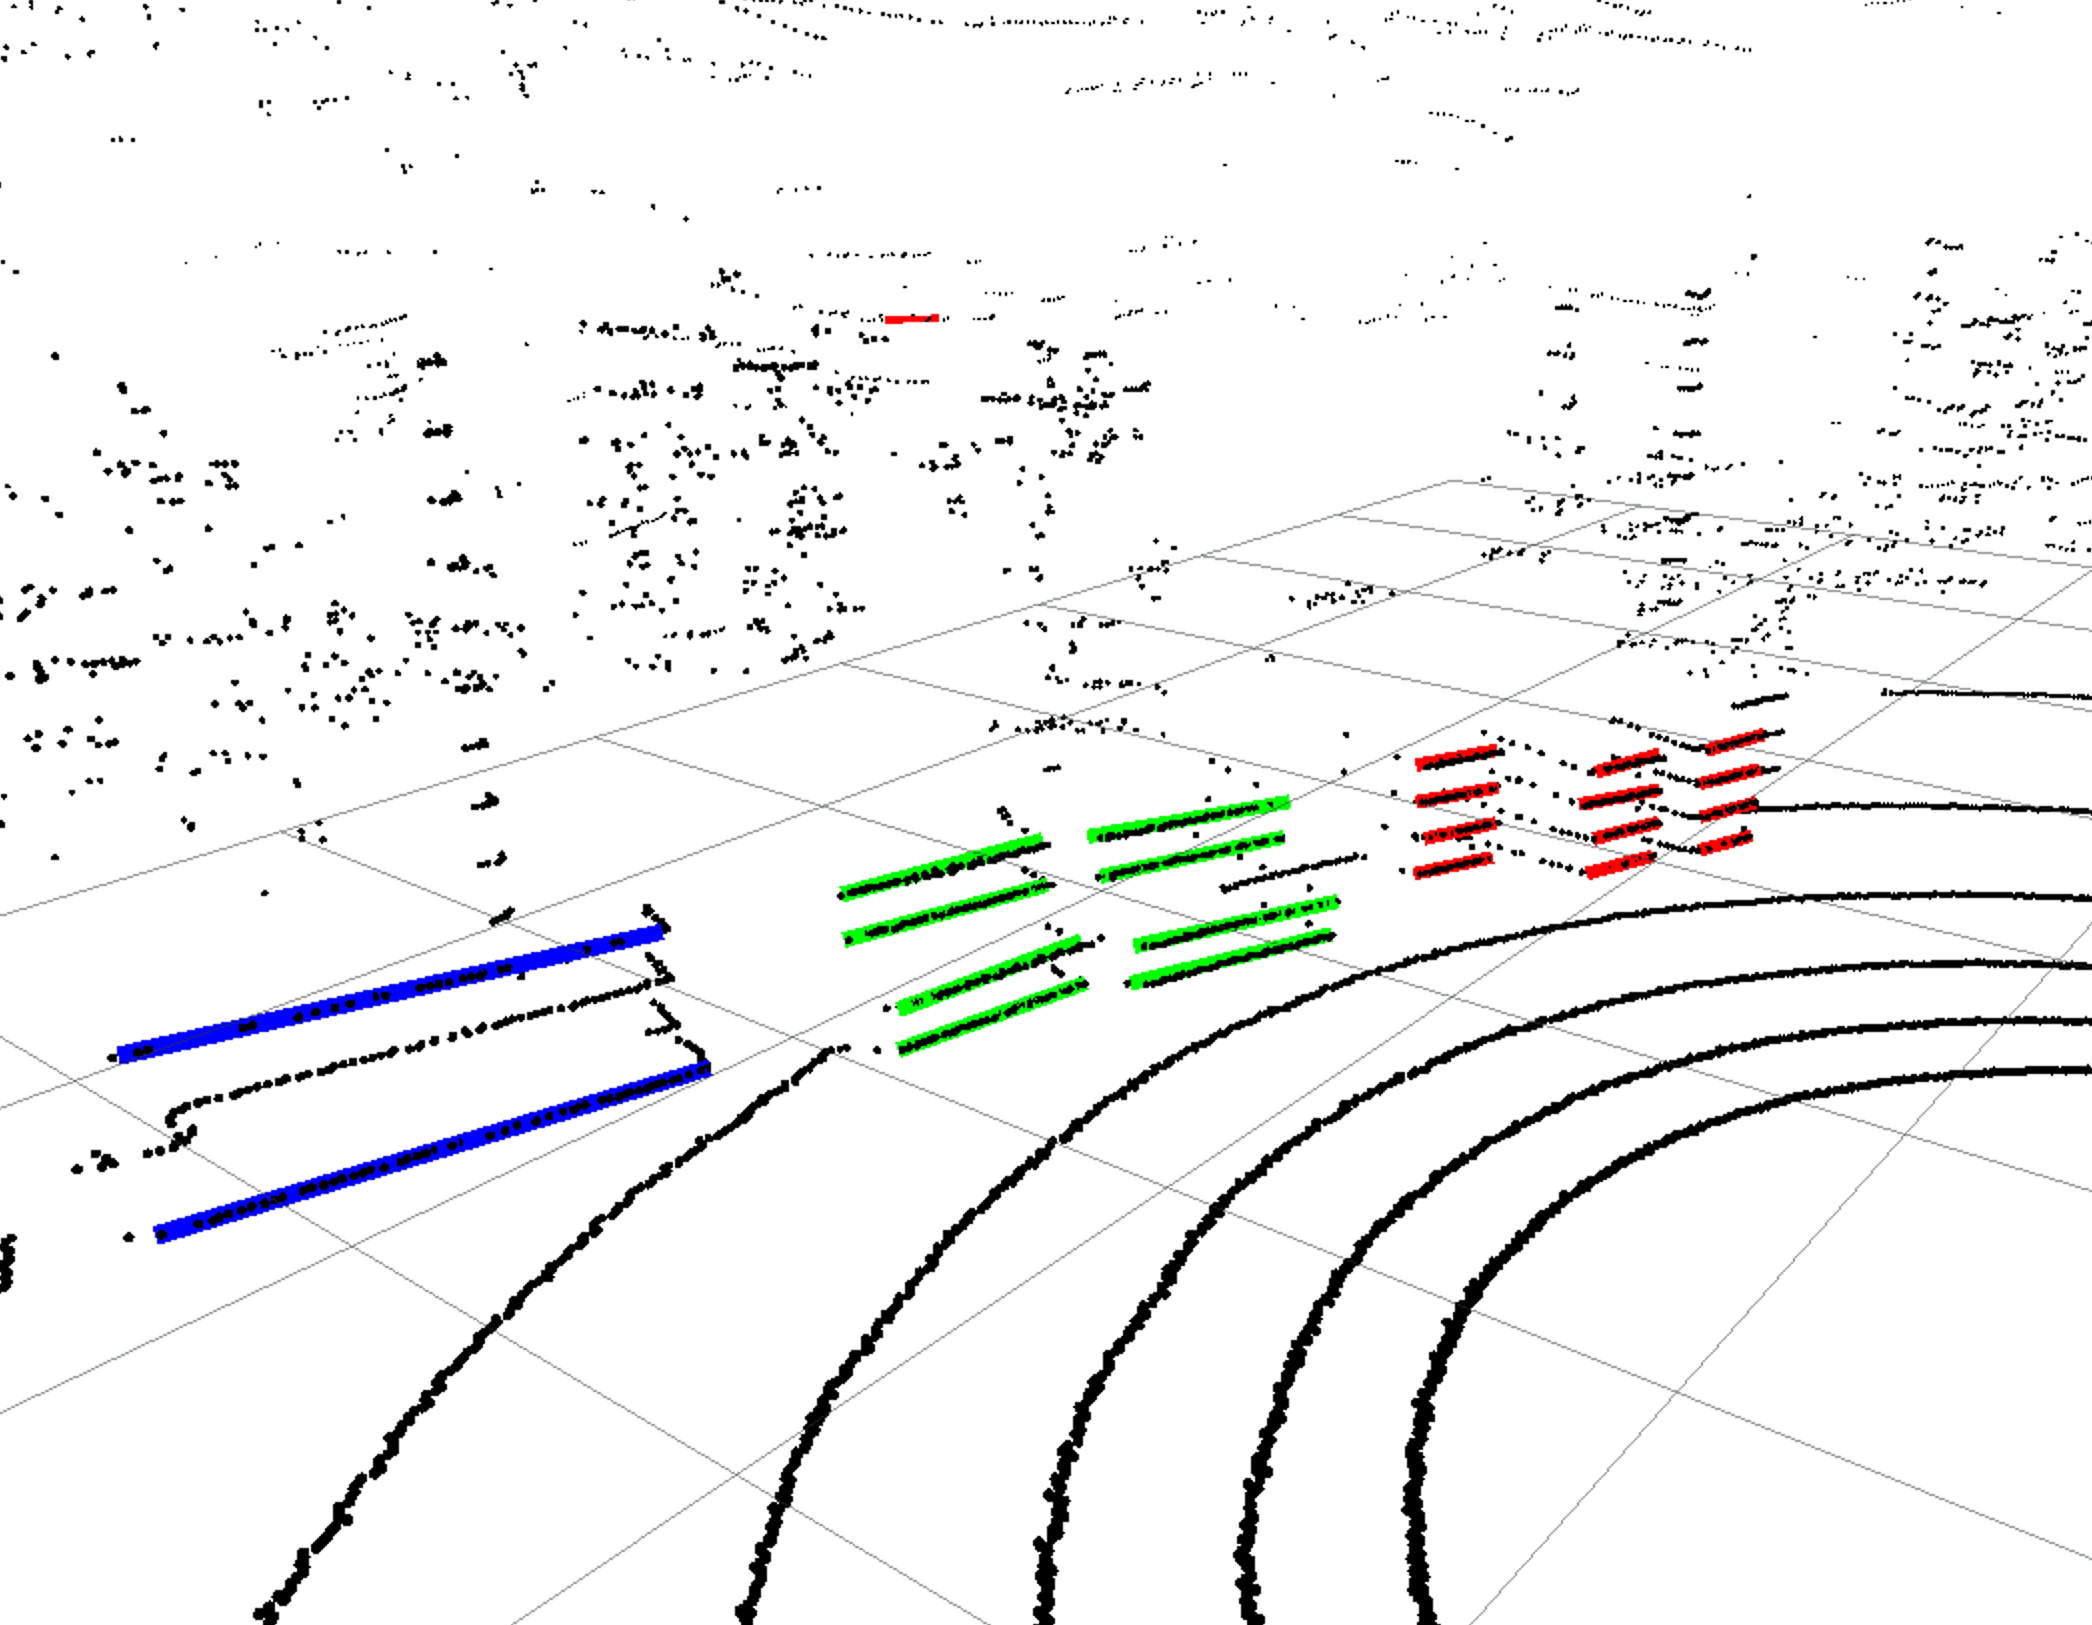
\includegraphics[scale=0.43]{fig/segments}
\caption[Line segmentation visualization]{Visualization of line segmentation. In the figure, it is evident that the bricks are well detected. This detection is done approximately from a distance of $3$m. There is one false positive detection visible behind the brick piles on a tree. The squares in the grid has $1\si{m}^2$.}
\label{fig:segments}
\end{figure}


\section{Pile detection}
\label{sec:pile_detector}
The pile detector uses one of the simplest versions of the EM algorithm. As a model for the pile is applied 2D multivariate Gaussian distribution with variance fixed to one. Although this model is not an accurate description of the detection probability, it has other advantages already discussed in previous chapters. It is easy to work with, and it converges to the global optimum very well. Only the mean value is optimized, and it should converge into the center of the pile. The stopping criterion for the algorithm is solely the number of iterations. The robot is a realtime system, and there are strict demands for meeting a deadline. 

There are further requirements for a hypothesis to be declared as a pile after the optimization is done. We look around the proposed center in a one-meter radius, and we inspect all bricks found in this area. All the following conditions must be fulfilled for segments in a pile:
\begin{enumerate}[label=(\alph*)]
\item There are at least two unique heights ($z$ positions).
\item There are at least two unique places ($(x,y)$ positions).
\item The difference between maximal and minimal height is smaller than the pile height.
\item The center of the pile is inside the arena.
\end{enumerate}
When these conditions are met, the hypothesis is declared as the pile and pushed into the symbolic map with high confidence. When at least one of these conditions is violated, then all the segments in this hypothesis are deleted, and the algorithm runs again until there are no more segments within the hypothesis radius. The condition (b) does not apply to the orange and blue pile because they have a different structure than the others. The whole procedure is shown in Algorithm \ref{alg:pile_detection}.
\begin{algorithm}[]
 \KwData{segments}
 \KwResult{pile\_position}
\While{True}{
	pile\_position = fit\_em(segments)\;
	pile\_segments = segments\_in\_pile(pile\_position, segments)\;
	\If{pile\_segments.size() $< 2$}{
		return None\;	
	}
	\eIf{is\_pile(pile\_segments)}{
		return pile\_position\;
	}{
		segments.delete(pile\_segments)\;
	}
} 
 \caption{Algorithm to obtain pile centers.}
 \label{alg:pile_detection}
\end{algorithm}

\begin{figure}[H]
\centering
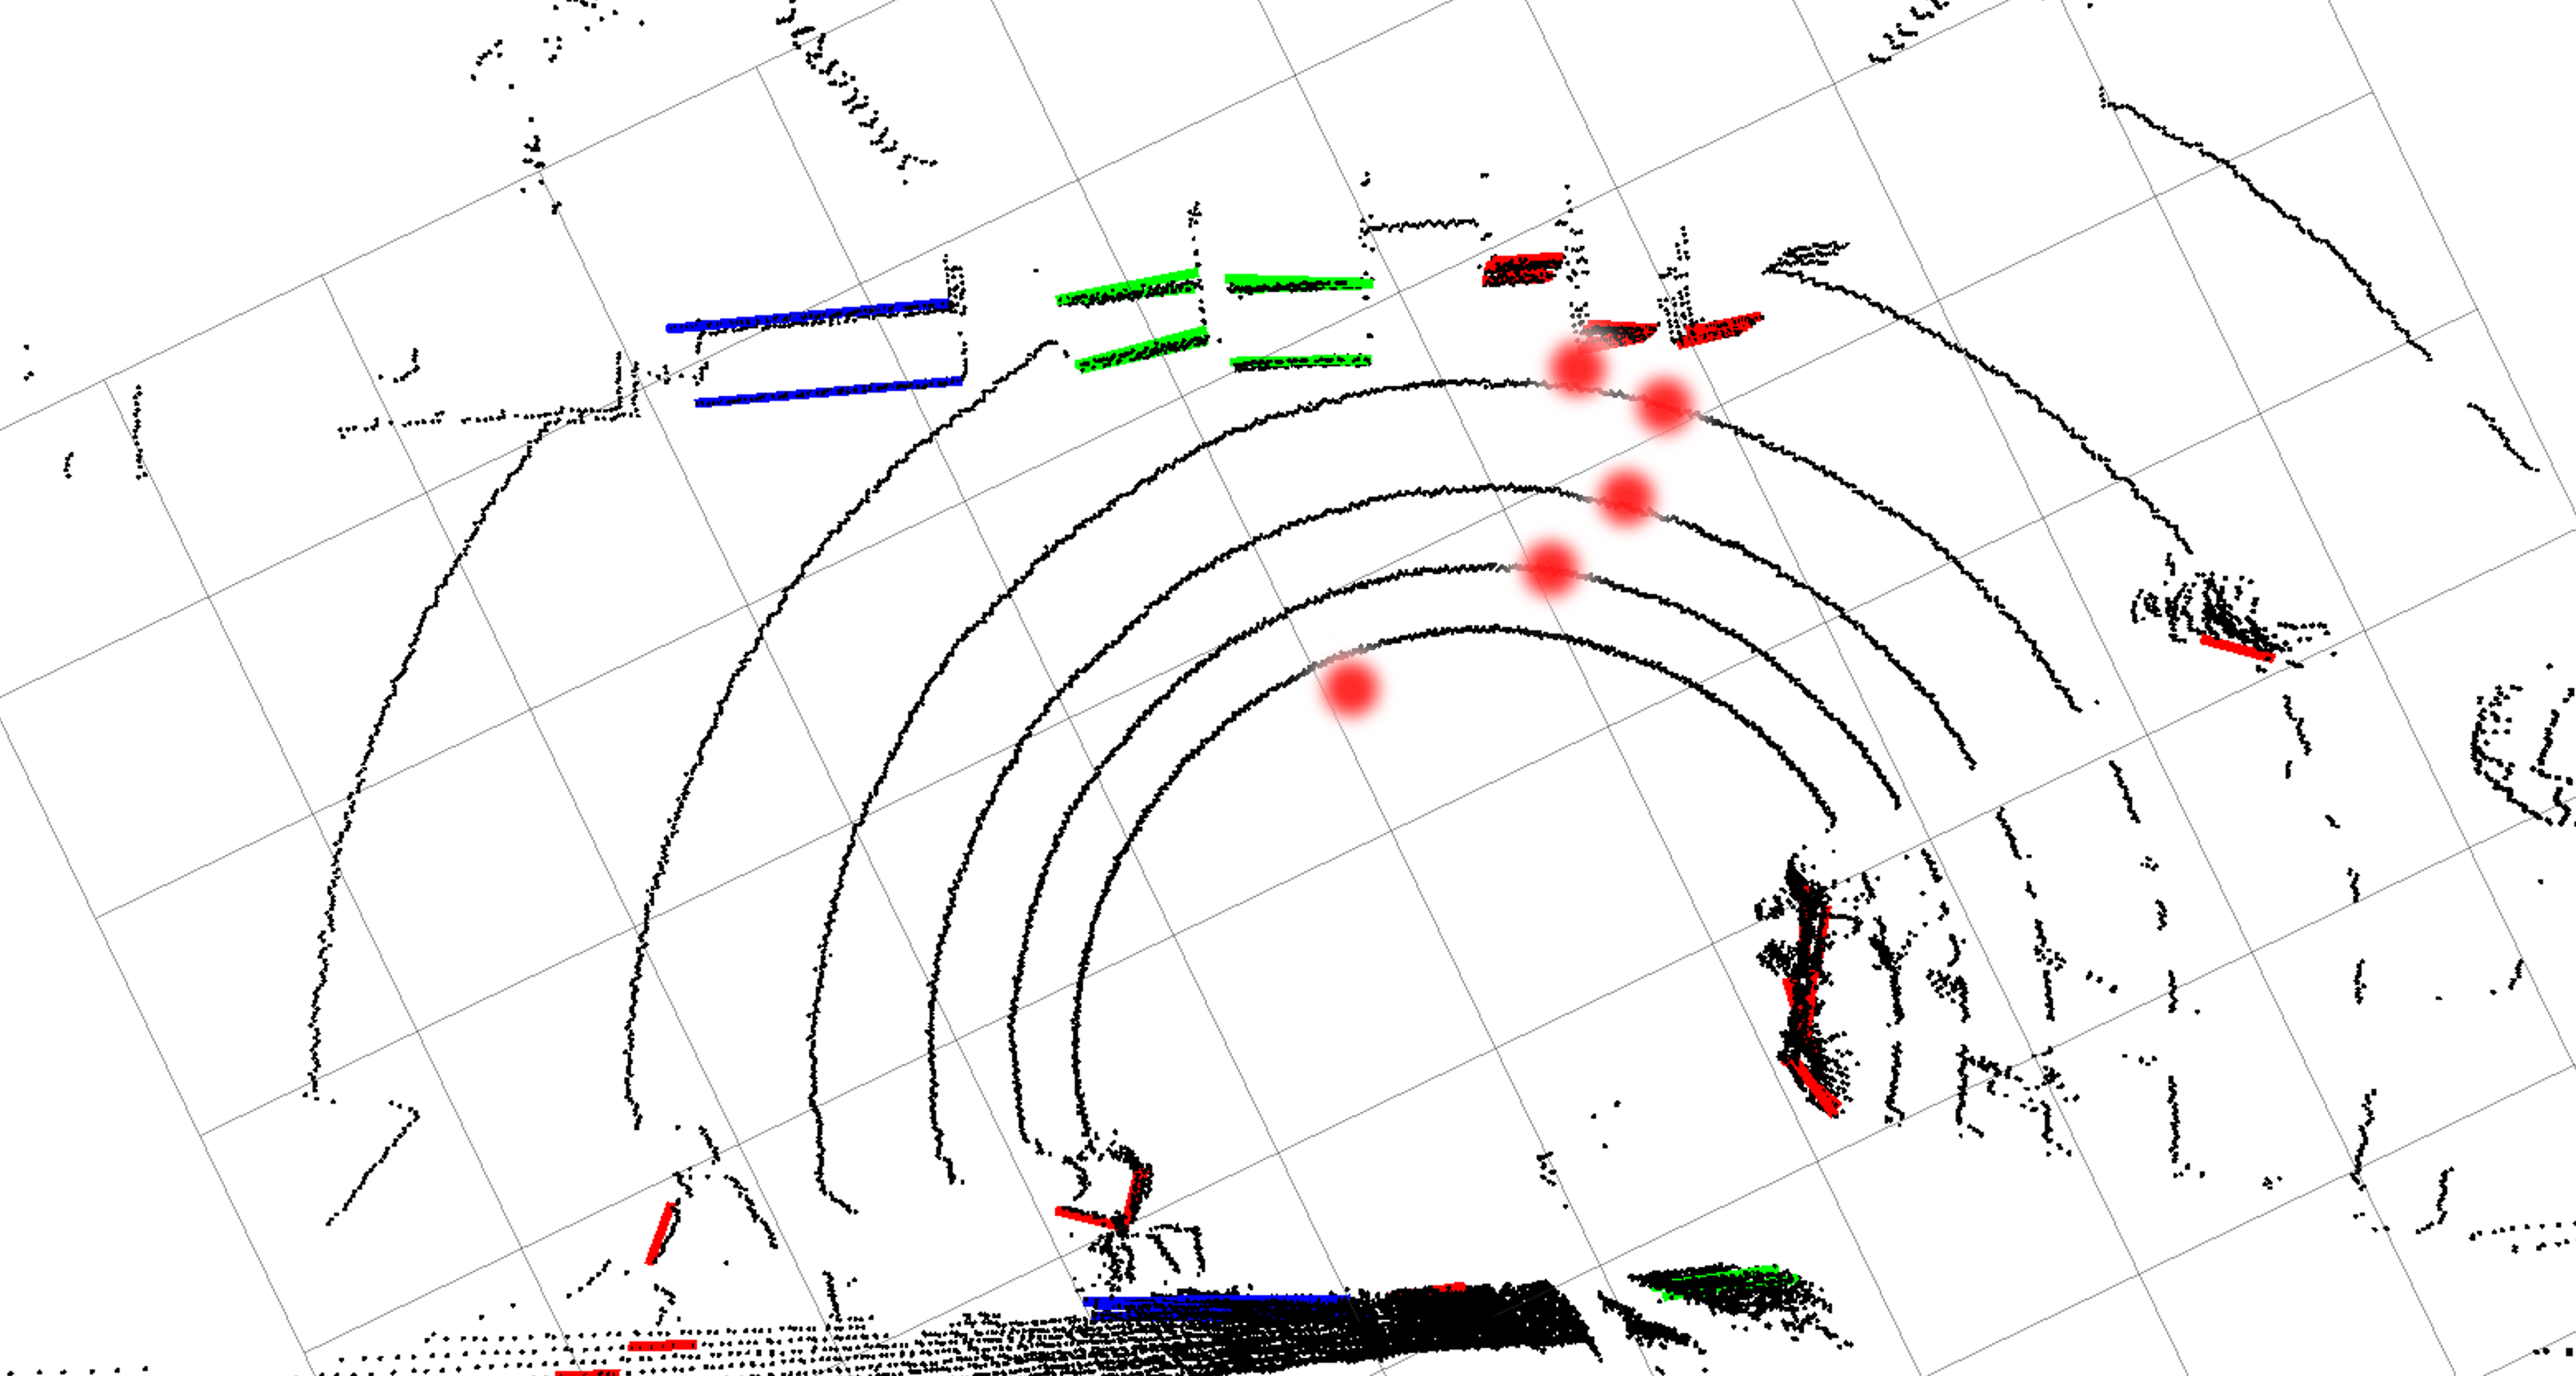
\includegraphics[scale=0.3]{fig/em_algo.png}
\caption[Em Algorithm in pile detector]{Several steps of the EM algorithm for the red pile. Colored lines are the visualized segments the same as in Figure \ref{fig:segments}. Red dots show subsequent positions of the mean value of multivariate Gaussian. Although there are many false positives, especially at the bottom of the picture, the pile model ensures that the algorithm converges to the correct place.}
\label{fig:em}
\end{figure}


\section{Pattern fitting}
As shown in Figure \ref{fig:flowchart}, the last step of the detection pipeline is pattern fitting. It is also visible that there are two types of input into this last step. Each input is used for a different type of pattern fitting. In the previous two sections, it was described how to generate candidates with different levels of confidence. This section describes how these candidates can be used for generating actual positions and how information about the spatial distribution of bricks can be exploited for the detection. The exact position of each pile and even each brick is visible in Figure \ref{fig:piledef}. The pattern in which the bricks are stacked has three degrees of freedom - position $(x, y)$ and rotation $\phi$. The goal of the pattern fitting is to find the values of these parameters in the map frame.

\subsection{Brick fitting}
The first type of fitting uses detected 3D positions of individual bricks obtained in a pile detector. The pattern defines the position of each brick, which can be detected by the lidar sensor. The next step is to generate a hypothesis that aligns this pattern with the measured positions of bricks. This step utilizes the RANSAC algorithm. Firstly we draw two different bricks from the detected set of bricks. Secondly, the correspondences are used to find the transformation - two correspondences are enough to generate the hypothesis (rotation matrix $\bm{R}$ and translation vector $\vec{t}$). The brick types (colors) and brick $z$ positions are used as the correspondences. Also, we know that the distance between corresponding pairs should match. Otherwise, it would be incorrect correspondence. Lastly, we measure the cost of the hypothesis. When the bricks are stacked into the pattern with reasonable precision, it is possible to fit the pile with average brick error down to $\pm 3$cm. After such an observation, we set the inlier distance $d_{inlier}$ to $5$cm. The algorithm is stopped after a certain number of iterations. The result is passed only if all detected bricks are inliers.

\subsubsection{Hypothesis ambiguity}
We cannot properly test the hypothesis when there are not enough bricks found. In addition, we can see the pile from behind, which renders two different patterns to match. For this reason, at least five detected red bricks are required to start the brick fitting. As shown in Figure \ref{fig:ambiguity}, even with four detected red bricks, the hypothesis can be easily fitted incorrectly. All conditions which can start fitting the hypothesis from front view are listed below:
\begin{enumerate}[label=(\alph*)]
\item 5 red bricks detected.
\item 3 green bricks detected.
\item 4 bricks of at least two colors detected.
\end{enumerate}
For the view from behind, only the condition (c) is sufficient.
\begin{figure}[H]
\centering
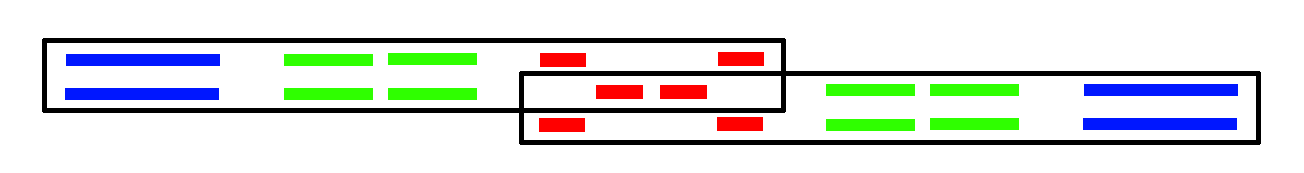
\includegraphics[scale=0.3]{fig/ambiguous.png}
\caption[Hypothesis ambiguity]{Two possible hypothesis which can be generated by four red bricks in their intersection are visualized in the black rectangles. This is a top view of detection from the front, so it is not visible that all red bricks are in two layers.}
\label{fig:ambiguity}
\end{figure}

\subsection{Cluster fitting}
The second type of fitting polls the clusters from the symbolic map and utilizes the confidence of clusters and their spatial distribution. For the RANSAC algorithm, a hypothesis using only four clusters would be too sparse to fit reliably. Because of this reason, the cluster fitting is done by the EM algorithm. As in pile detection, multivariate Gaussian distribution is used to represent the pile, but this time, the model takes into account relationships between positions of the piles. We define the probability model as follows:
\begin{equation}
P(\vec{x}_m) = \mathcal{N}_m(\vec{x}_m; \vec{\mu} + k_m\vec{v}; \bm{\Sigma_m}),
\label{eq:prob}
\end{equation}
where $m$ is pile (color) index, and $M$ is an absolute number of colors, $\vec{x}_m$ is a measurement of color $m$, $\vec{\mu}$ is mean value of the whole model, $\bm{\Sigma_m}$ is a covariance matrix, $k_m$ is scalar multiplier unique for each pile and $\vec{v}$ is defined as:
\begin{equation}
\vec{v} = \begin{bmatrix}
\cos \phi \\
\sin \phi
\end{bmatrix},
\end{equation}
where $\phi$ is the rotation of the model. This definition of the model ensures that all piles (Gaussians) are in line with a distance defined by multiplier $k$. How such a model could look like is visualized in Figure \ref{fig:mnd}.

\begin{figure}[H]
	\centering
	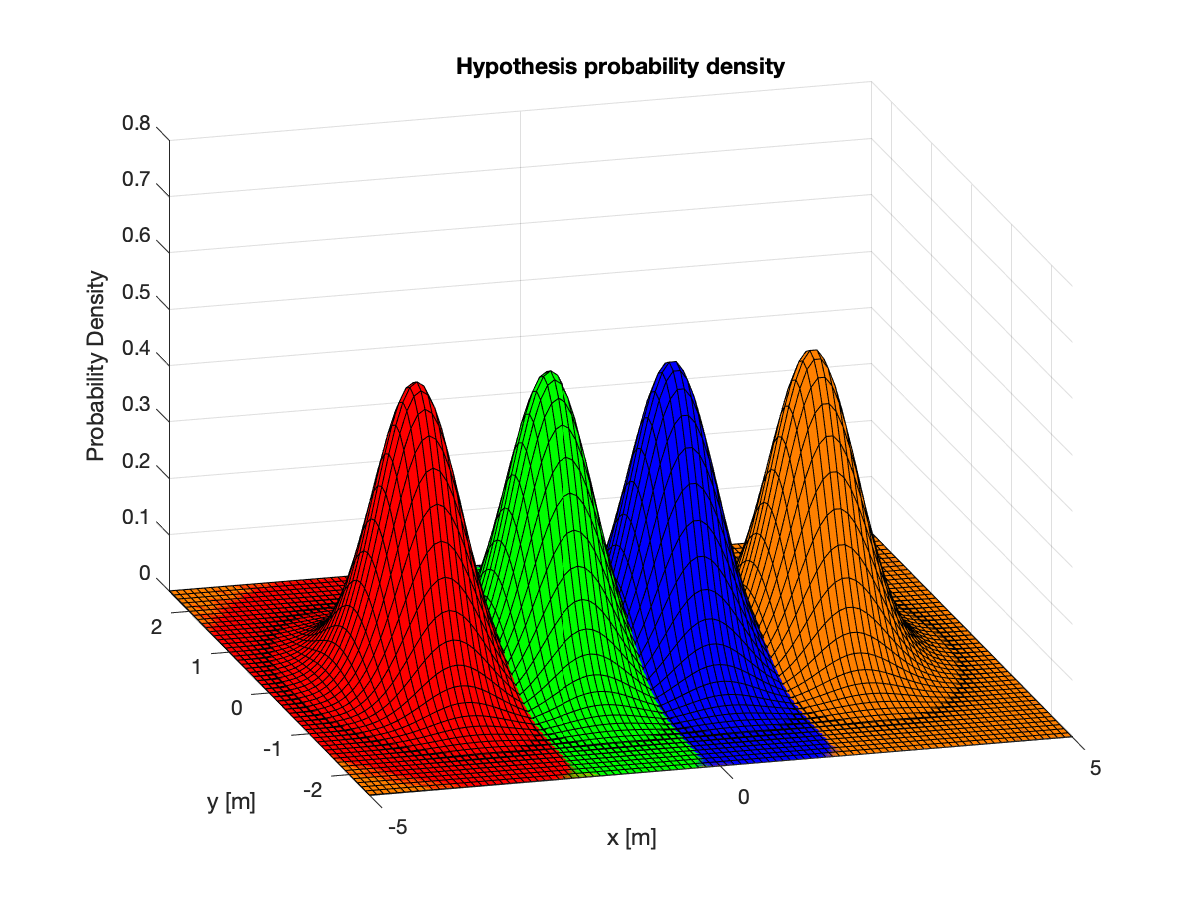
\includegraphics[scale=0.55]{fig/model_mnd.eps}
	\caption[Hypothesis ambiguity]{Example of a probability density function, which can be described as model \ref{eq:prob}. This particular model was created using $\vec{k}_{pile}$ from the Table \ref{tab:constants}, $\mu = [0, 0]$, $\phi$ = 0 and $\bm{\Sigma} = 0.3\bm{E}$, where $\bm{E}$ is identity matrix of size $2$.}
	\label{fig:mnd}
\end{figure}

 Now we want to obtain the position and rotation of such a model based on real measurements. There is a closed-form solution for maximizing both terms, which can be found using the maximum likelihood estimate. For mean value, the derivation is very similar to multivariate Gaussian:
\begin{align}
\frac{\partial \log\mathcal{L} }{\partial \vec{\mu}_m} &=  \bm{\Sigma}^{-1}_m \sum_{n = 1}^{N_m} (\vec{x}_{m_n} - \vec{\mu} - k_m \vec{v}), \\
\vec{\mu_m} &= \sum_{n = 1}^{N_m} \frac{\vec{x}_{m_n} - k_m \vec{v}}{N_m}.
\end{align}
Further, it is necessary to derive MLE for rotation $\phi$, which is hidden inside vector $\vec{v}$. For simplicity the matrix equation is now split into one part for each of two dimensions:
\begin{align}
\frac{\partial \log\mathcal{L}_x }{\partial \phi_m} &= \frac{1}{\sigma^2_x} \sum_{n=1}^{N_m} (x_{m_n, x} - \mu_x - k_{m, x} \cos \phi) \left( -k_{m,x} \sin \phi\right),  \\
\frac{\partial \log\mathcal{L}_y }{\partial \phi_m} &= \frac{1}{\sigma^2_y} \sum_{n=1}^{N_m} (x_{m_n, y} - \mu_y - k_{m, y} \sin \phi) k_{m,y} \cos \phi.
\end{align}
Likelihood derivative is now set equal to zero to find the extremes for each dimension:
\begin{align}
\cos \phi_m &= \frac{1}{k_{m, x}N_m} \sum_{n = 1}^{N_m} \left(  x_{m_n, x} - \mu_x \right)  , \\ 
\sin \phi_m &=  \frac{1}{k_{m, y}N_m} \sum_{n = 1}^{N_m} \left(  x_{m_n, y} - \mu_y \right)  .
\end{align}
Now it is possible to divide one equation by the other, use the basic relationship of trigonometric functions, and derive the final expression for maximizing the rotation $\phi$:
\begin{align}
\phi_m &= \arctan \left( \frac{\dfrac{\sum_{n = 1}^{N_m} \left( x_{m_n, y} - \mu_y \right)}{k_{m, y}N_m} }{ \dfrac{\sum_{n = 1}^{N_m} \left( x_{m_n, x} - \mu_x \right)}{k_{m, x}N_m} }\right).
\end{align}
Although the expression can be further simplified, in this form, it is easier to weight each data sample by the expectation $\gamma$. Also, it is necessary to consider the contribution of each color to the pile model. This can be done in two ways. One possibility is to set an equal contribution to each data sample. In our case, this could lead to bias towards the most detected color (usually red). Therefore we set equal contributions to all colors instead of the samples. The final form used in the maximization step looks as follows:
\begin{align}
\vec{\mu} =& \sum_{m=1}^M \dfrac{1}{M}\sum_{n = 1}^{N_m}  \vec{\gamma}_{m_n} \left( \vec{x}_{m_n} - k_m \vec{v} \right) , \\
\phi = \arctan & \left( \dfrac{\sum_{m=1}^{M} \dfrac{\sum_{n = 1}^{N_m} \gamma_{m_n, y}(x_{m_n, y} - \mu_y)}{k_{m, y} } }{\sum_{m=1}^{M} \dfrac{\sum_{n = 1}^{N_m} \gamma_{m_n, x} (x_{m_n, x} - \mu_x) }{k_{m, x}} }\right).
\end{align}
The method is demonstrated in Figure \ref{fig:em_pattern}. The expectation is calculated simply by evaluating the probability of sample $P(\vec{x}_m)$ as in equation \ref{eq:prob}. Results can be further improved when the confidence of the sample is used as the prior probability.

\begin{figure}[H]
	\centering
	\begin{subfigure}{0.49\textwidth}
		\centering
		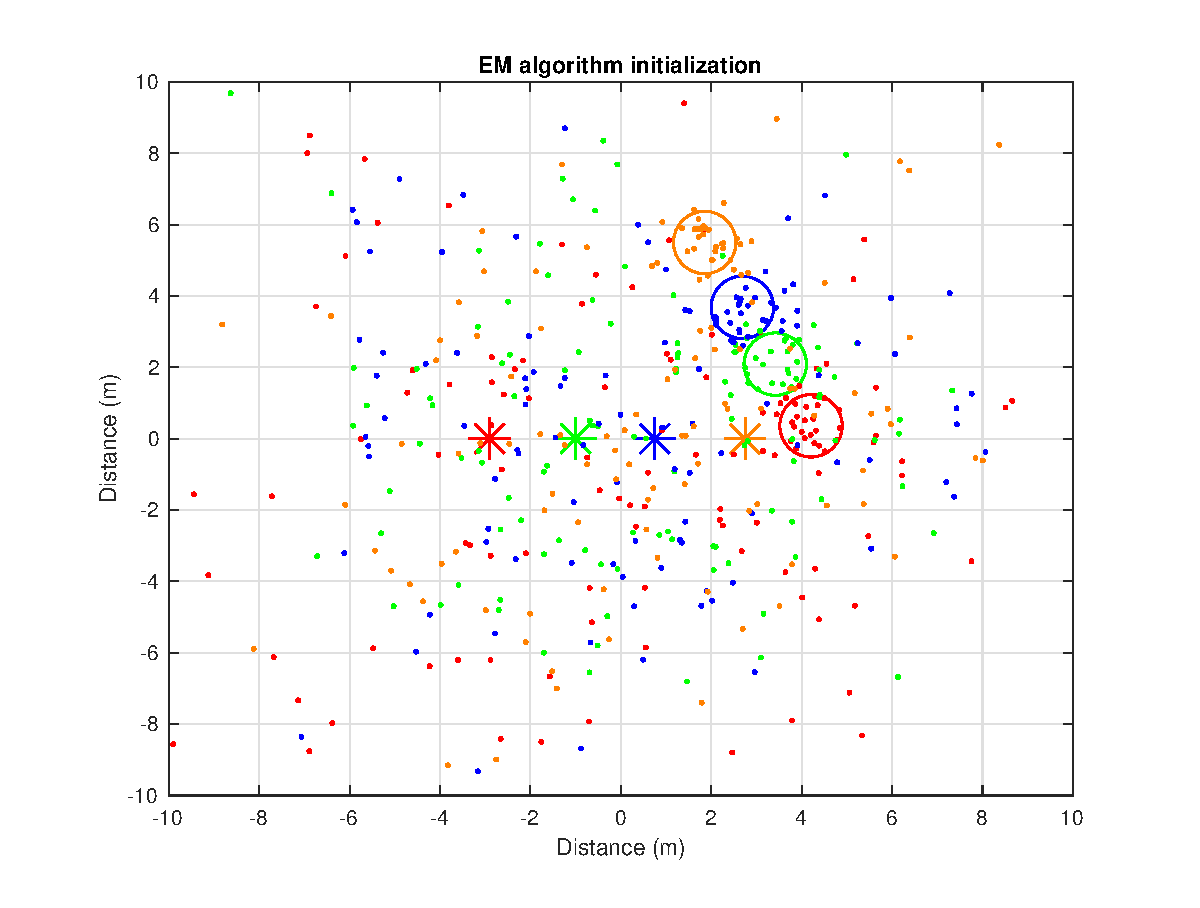
\includegraphics[scale=0.43]{fig/em_init.eps}
	\end{subfigure}
	\begin{subfigure}{.49\textwidth}
		\centering
		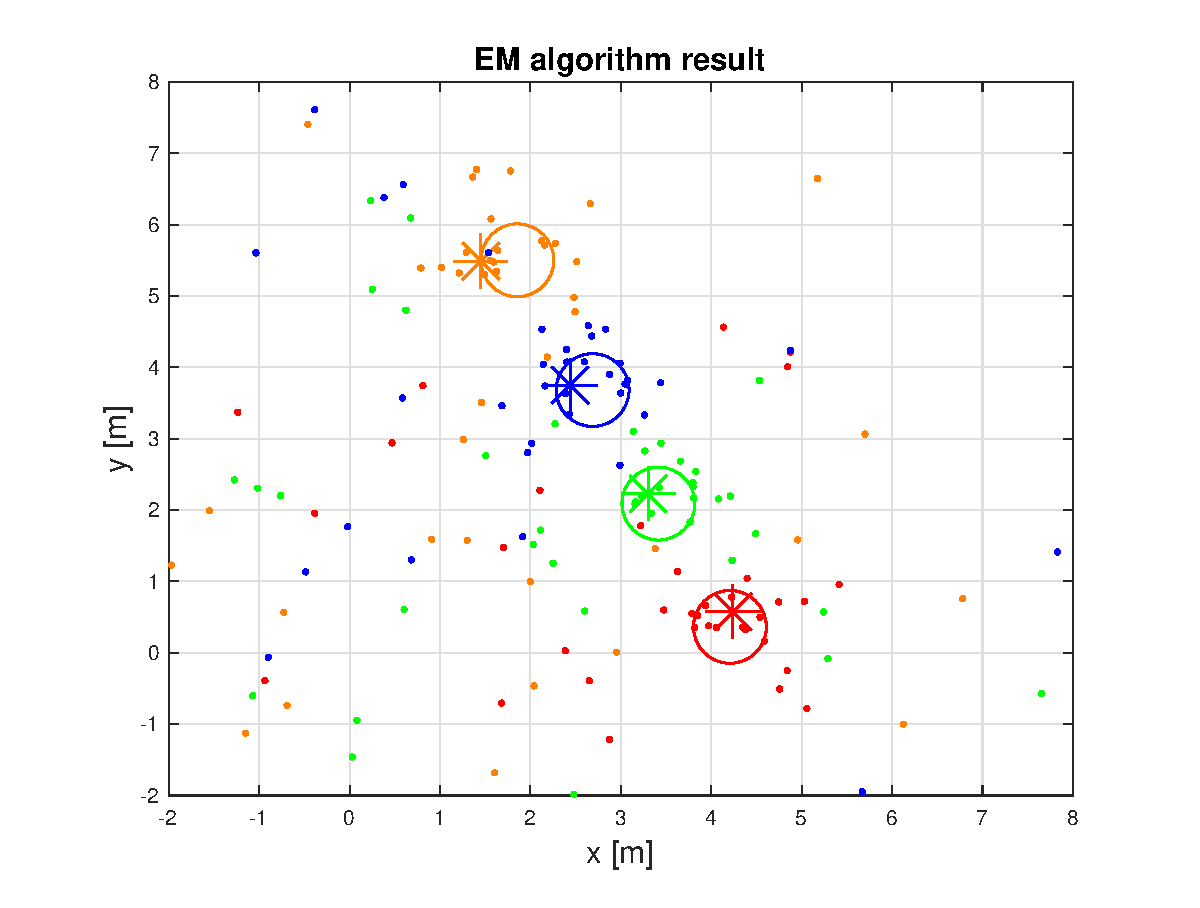
\includegraphics[scale=0.43]{fig/em_result.eps}

	\end{subfigure}
	
	\caption[EM pattern fitting]{In the pictures, the pattern fitting using the EM algorithm is visualized. On the left there is algorithm initialized with parameters $\vec{x}=(0, 0)$ and $\phi=0$. Stars mark the algorithm estimate. Points are generated by sampling multivariate Gaussian distribution. The model was sampled with parameters $\vec{x}=(3, 3)$ and $\phi=2$ to create the desired pattern of points. Positions of sampled piles are marked as circles. At the end of the procedure, all parameters are found correctly.}
	\label{fig:em_pattern}
\end{figure}

\subsubsection{Convergence}
The unimodality of the model's likelihood was disrupted by adding the rotation parameter to Gaussians. Possible local optimum is shown in Figure \ref{fig:em_local}. Now there are no guarantees that the algorithm converges into the global optimum. That is a common issue of the EM algorithm when dealing with more complex problems. Many solutions to this issue were proposed. Very advantageous is that local optima are usually significantly worse in terms of likelihood than the global optimum. 

One way to avoid local optima is the deterministic annealing, which influences how the expectation is used in the maximization step \cite{ueda1998}. Another way how to escape local optimum is to apply perturbations to parameters of the model. In our case, it could be, for example, rotating the model by $180\degree$. A different approach would be a population-based em algorithm with multiple initializations or informed initialization. The latter is easily applicable in our case because the confidences of clusters could be used in the expectation step. 

Because we also have the formulas for gradient, it is also possible to use an arbitrary gradient ascend method instead of an MLE to maximize the likelihood of the model. The advantage of using the MLE for maximization step is that the algorithm converges very fast, and the computation is usually much faster than the computation of any gradient method.

\begin{figure}[H]
	\centering
	\begin{subfigure}{0.49\textwidth}
		\centering
		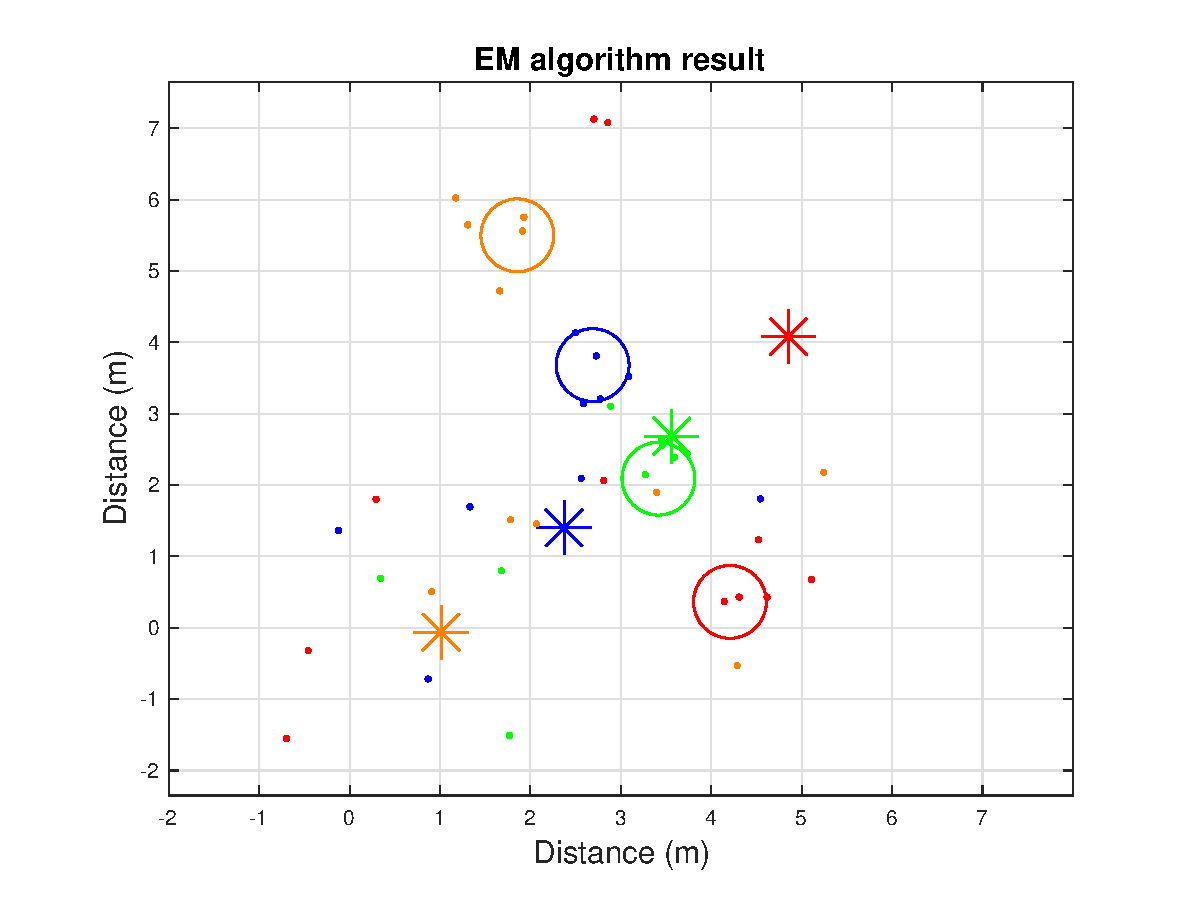
\includegraphics[scale=0.43]{fig/em_local.eps}
	\end{subfigure}
	\begin{subfigure}{.49\textwidth}
		\centering
		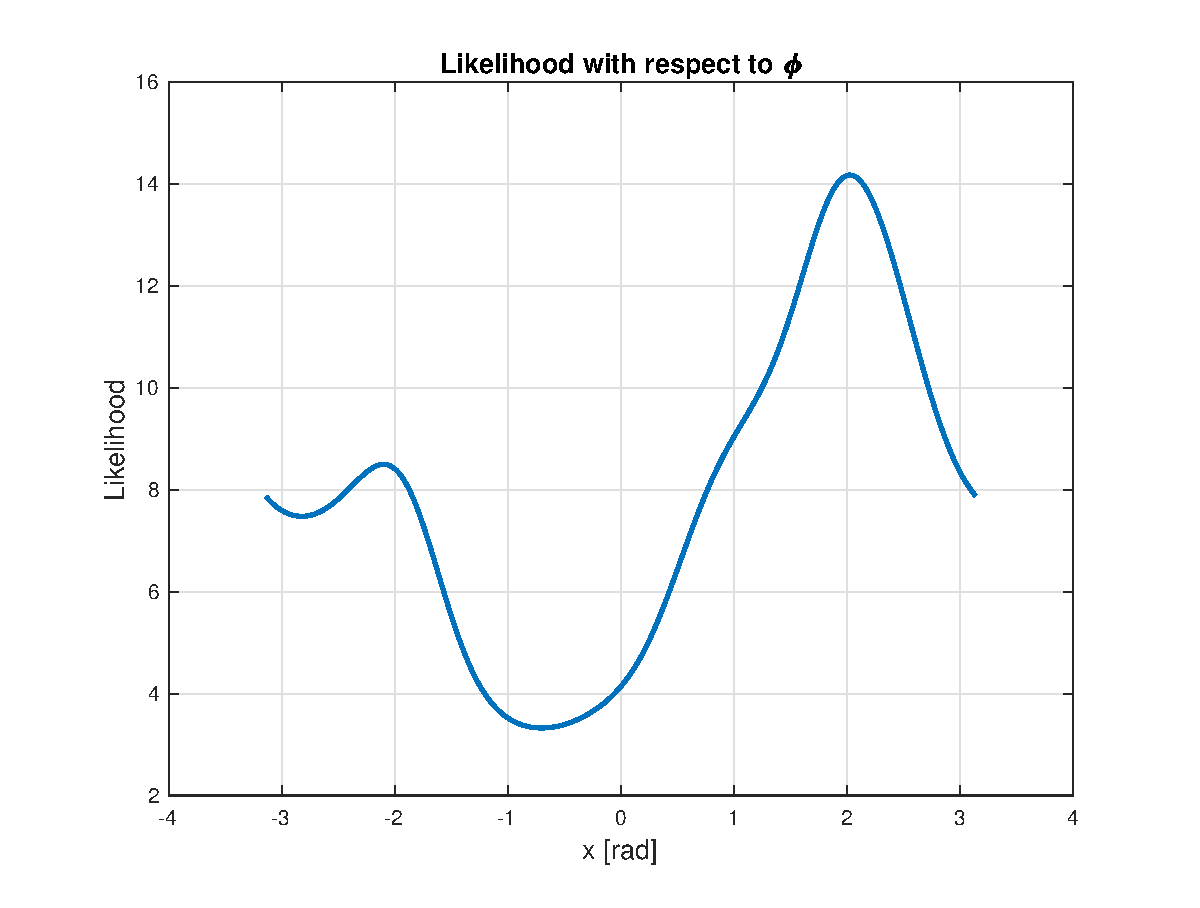
\includegraphics[scale=0.43]{fig/em_local_chart.eps}
		
	\end{subfigure}
	
	\caption[EM local optima]{When there are not enough samples, the EM algorithm is more susceptible to getting stuck in local optima, as shown on the left. The right picture shows how different rotations of the model with fixed mean influences the likelihood, and it also shows that there is a local maximum.  The likelihood is maximal when $\phi = 2$, which is the optimal rotation of the model.}
	\label{fig:em_local}
\end{figure}

\section{Arena exploration}
It is vital to emphasize on proper arena exploration. If all the interest points are not found, the robot can not proceed in completing the challenge. Except for the initial brick position, it is necessary to find also the destination where the bricks should be placed. This place is marked by the checker pattern in Figure \ref{fig:checker}. The only sensor which can detect the destination pattern is the camera. The big advantage is that the camera is mounted onto the arm so that it can be raised into height and turn around. As can be seen in Figure \ref{fig:detection_range}, the most limiting factor of the detection range is currently the UGV destination-pattern search.

\begin{figure}[H]
	\centering
	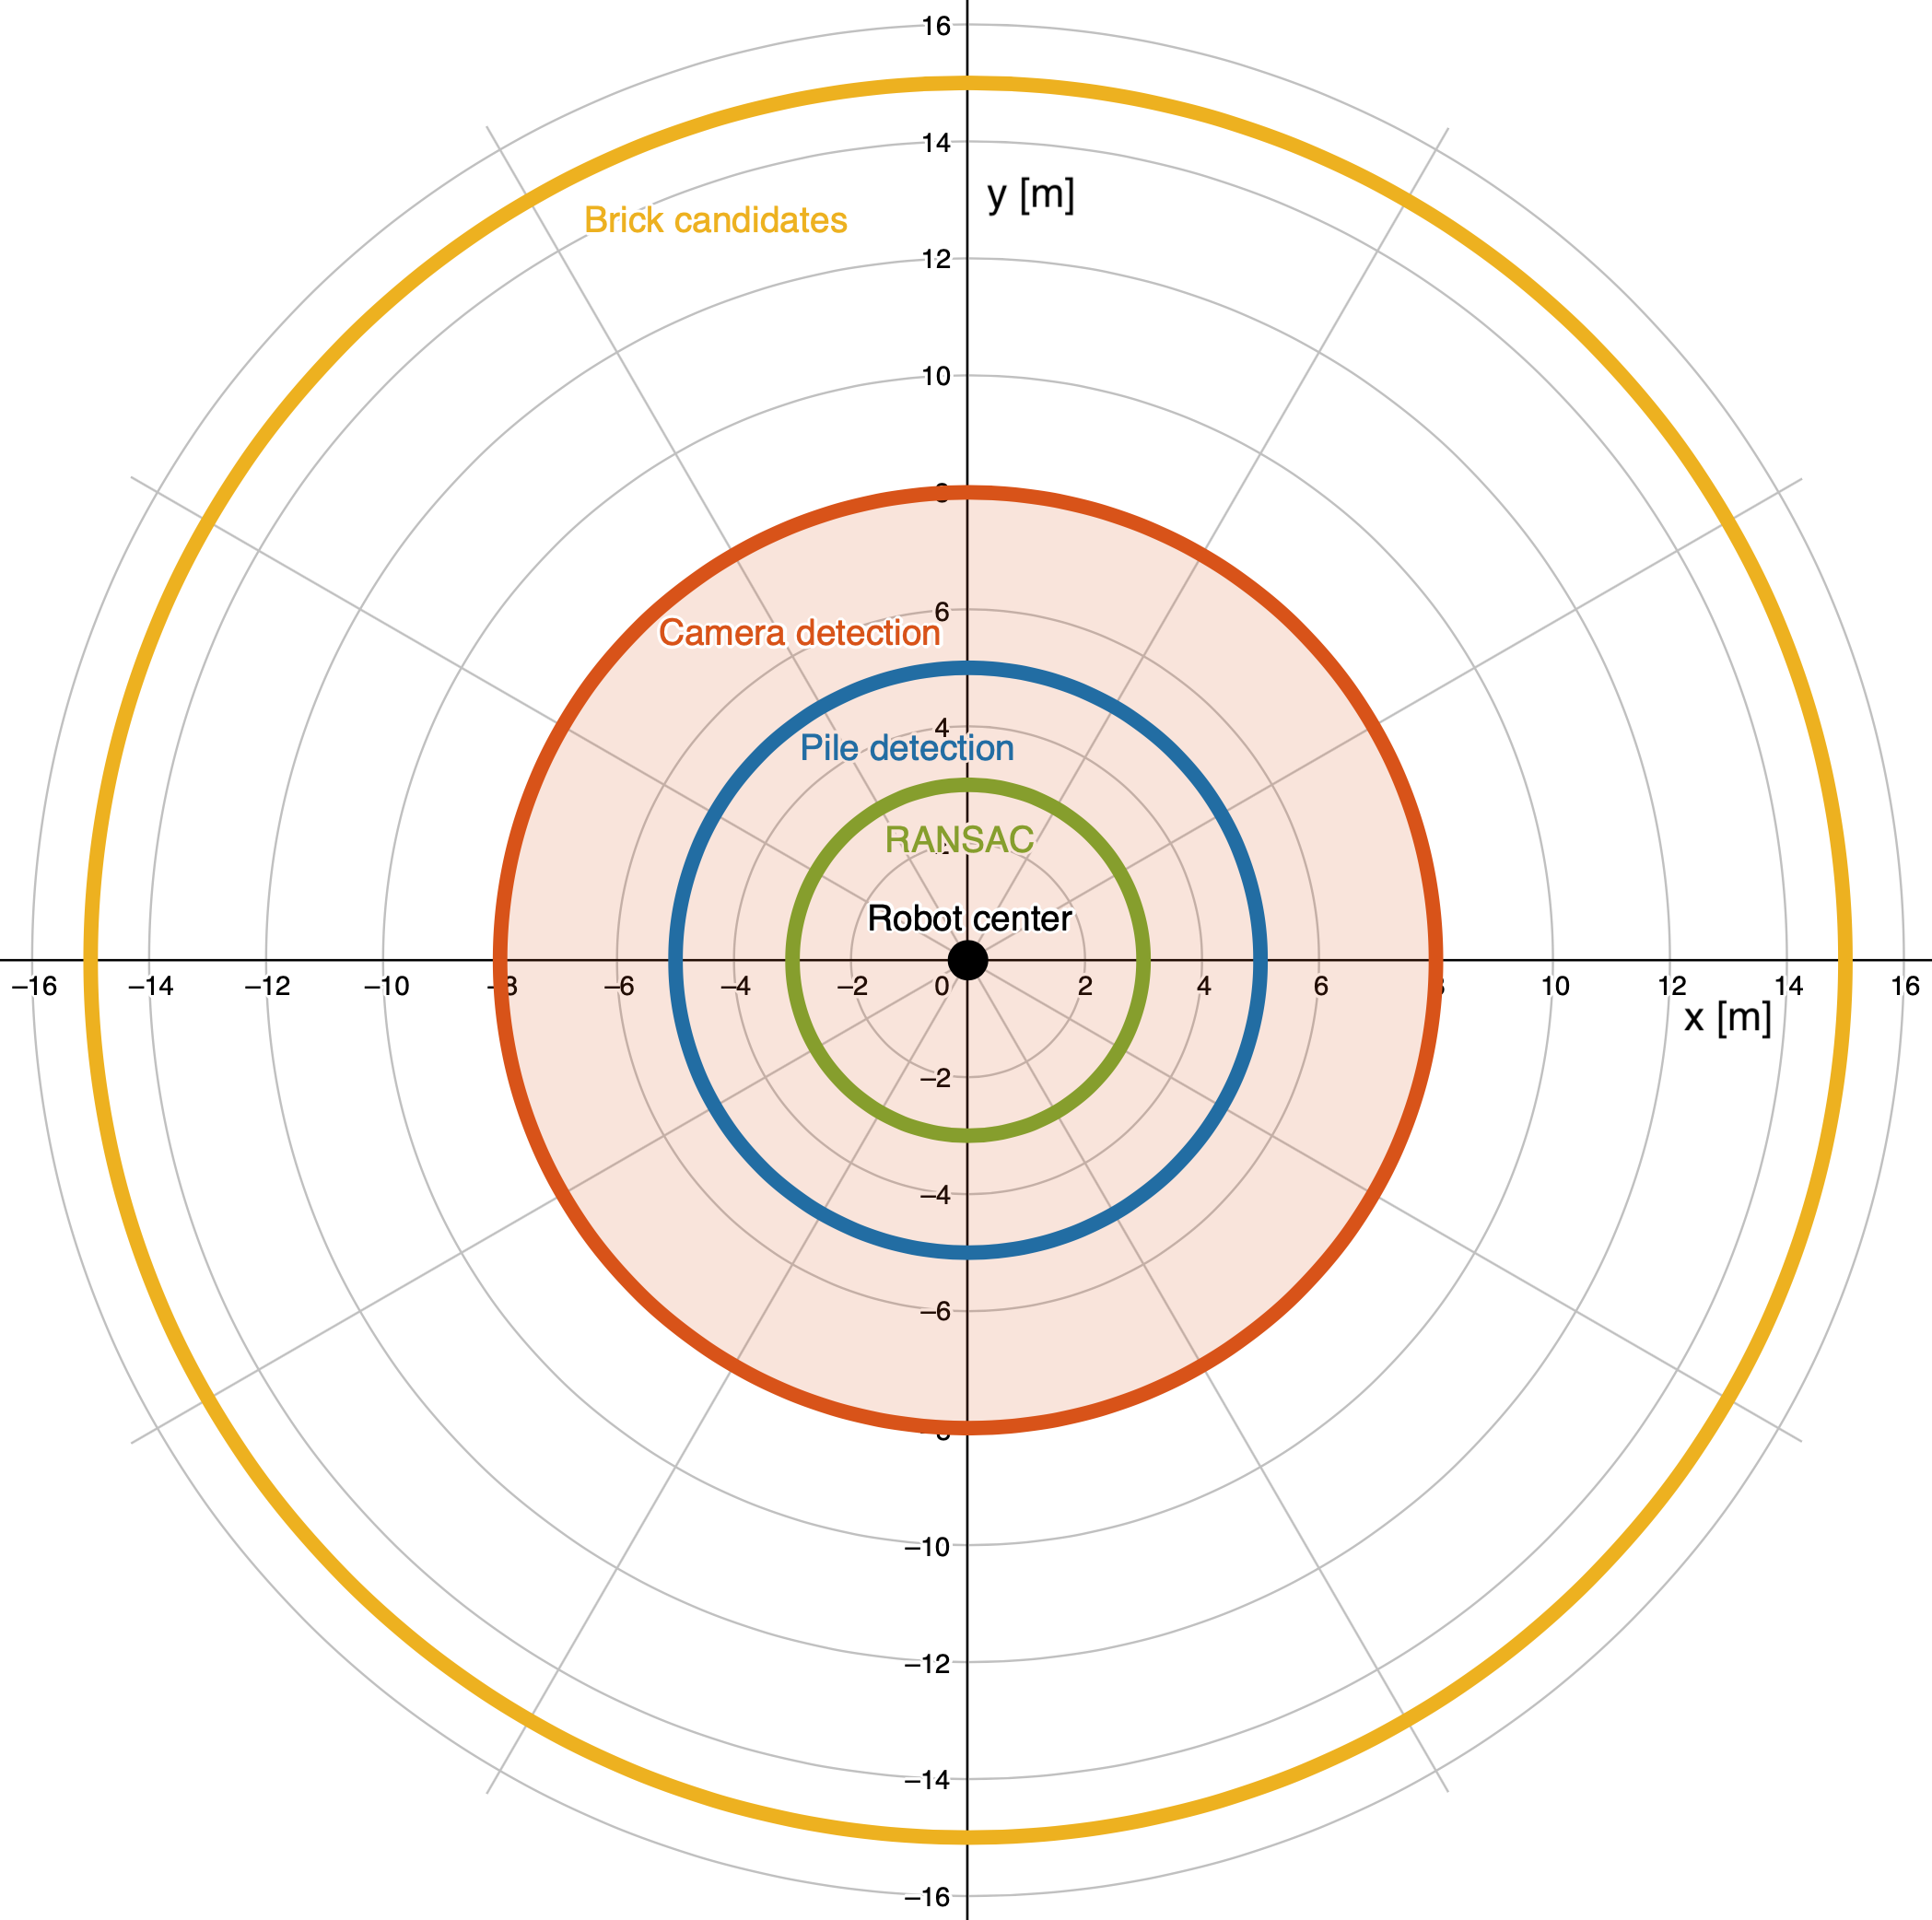
\includegraphics[scale=0.38]{fig/detection_range.png}
	\caption[Detection ranges]{In the picture, we see the range of each type of detection. Fitting the complete hypothesis with the RANSAC method (green) requires a high number of detected segments in piles, so the range is low - around $3$m. For detection of the pile (blue), just a few detected segments are required, so the detection range longer - around $5$m. The camera can obtain candidates for checker pattern (red) from the maximal distance of $8$m, which is the limit distance for exploration. From an even bigger distance, candidates for bricks (yellow) using the lidar sensor can be generated. The upper boundary can be even higher, but we set it manually to $15$m to reduce the number of false-positive detections.}
	\label{fig:detection_range}
\end{figure}

The waypoints of exploration movement should be generated so that circles cover the area of the whole arena with an $8$m radius. Generated waypoints in the arena are visualized in Figure \ref{fig:map_annot}. On each waypoint, the robot must stop, raise the arm, and look around with the camera. There are several reasons why camera detection cannot be done while moving. First of all, the arm can not be raised to the highest possible position while the robot is moving. Otherwise, it could get stuck or damaged. In addition, the motion blur of the camera would reduce the detection range even further. During camera detection, the robot must stay still, but the lidar detections can be done while moving. That can improve the detection range and speed because the robot can do measurement from many more different places. 

Whole map exploration is described in Algorithm \ref{alg:exploration}. The waypoints are ordered prior to this algorithm. How to order them is beyond the scope of this thesis. In the algorithm, it is visible that the method \textbf{start\_lidar\_detection} is non-blocking service, which just turns on the detector, whereas the method \textbf{do\_camera\_detection} is blocking service, which waits until the arm looks around with a camera and finishes the detection. This method is also the most time-consuming part of the loop.

\begin{figure}[H]
	\centering
	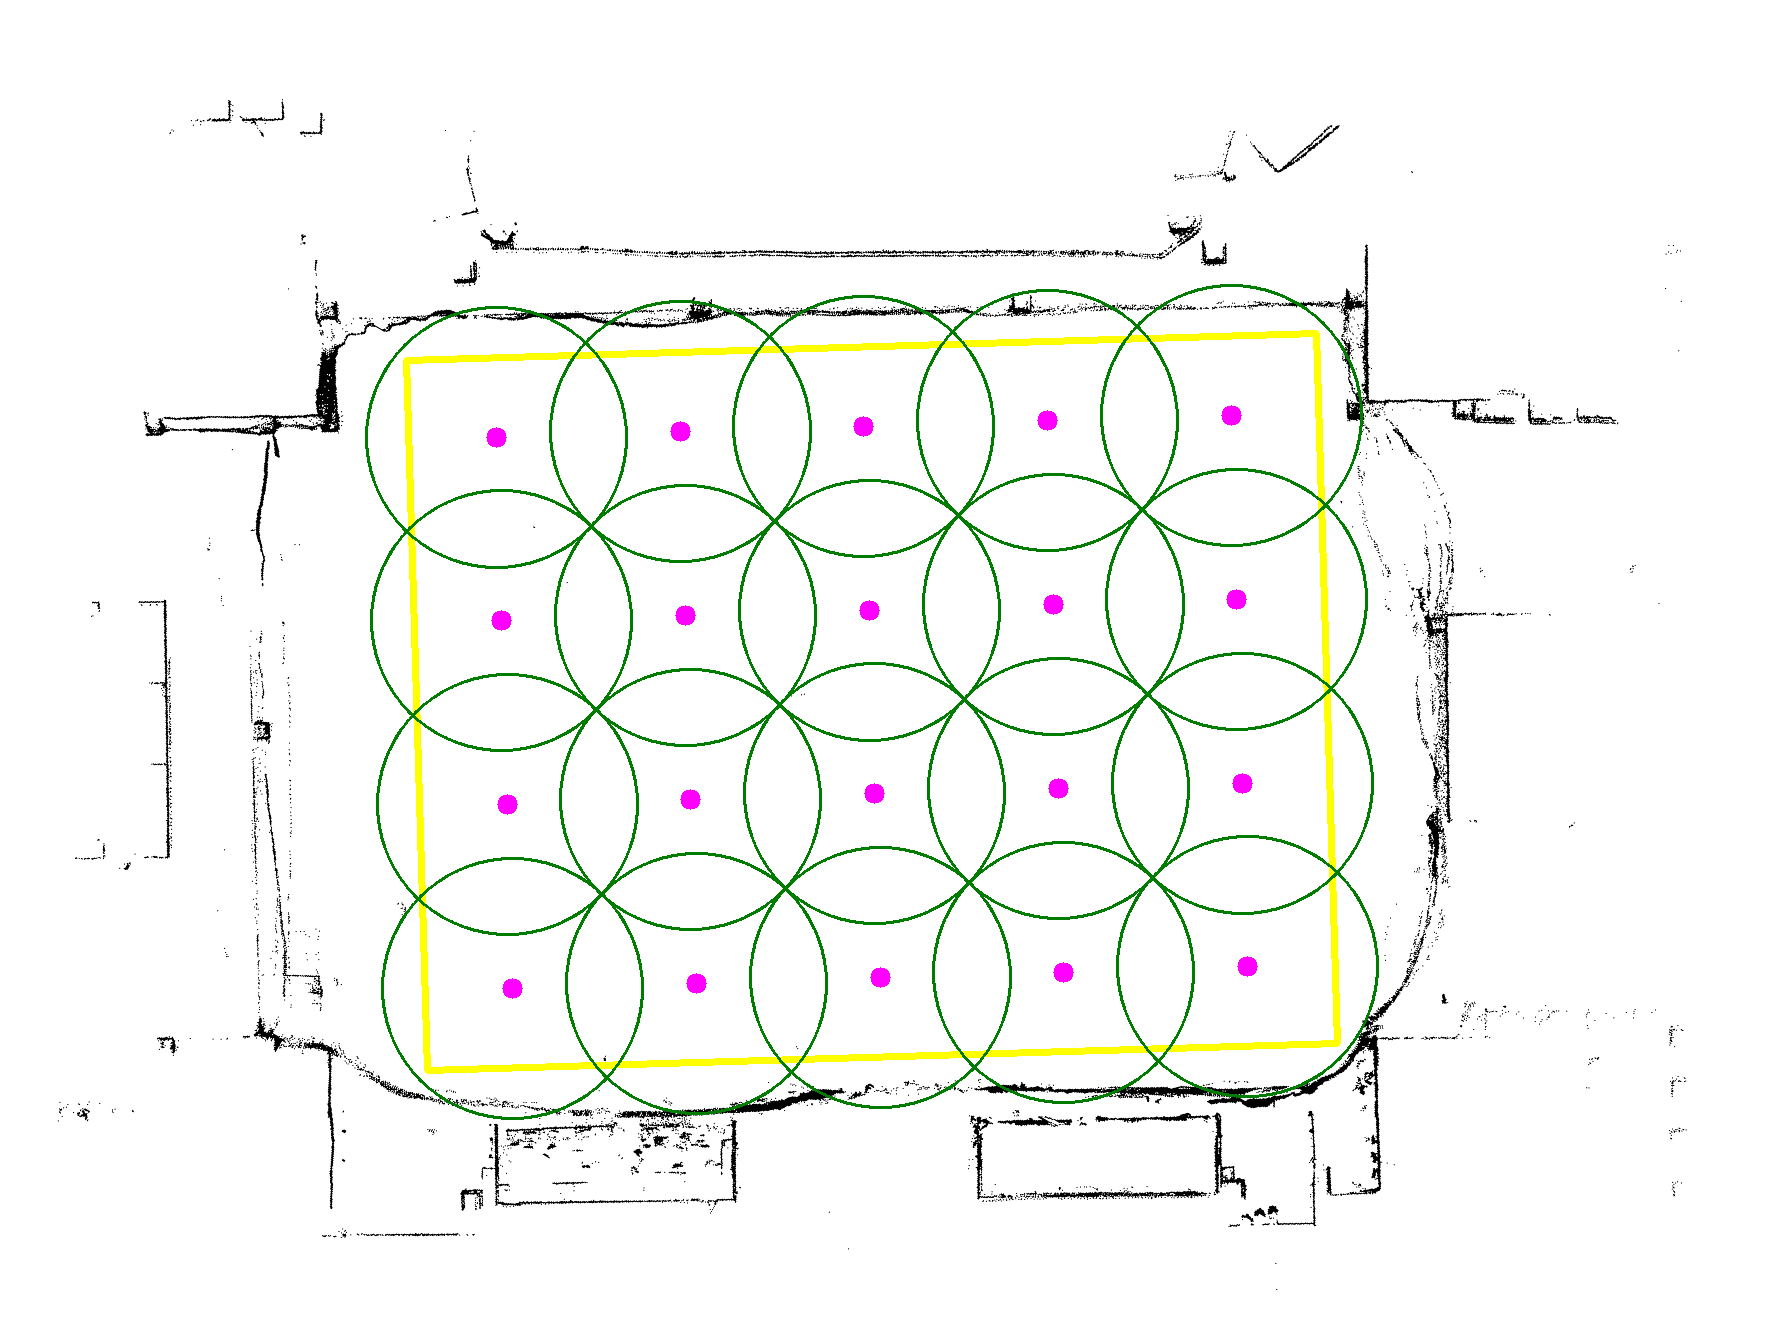
\includegraphics[scale=0.25]{fig/map_annotation.png}
	\caption[Generated waypoints]{Purple waypoints are places where the robot should stop and look around. Green circles are camera ranges from the corresponding place. In this figure, the waypoints are generated so that there is no unexplored area. That is usually not necessary since the objects of interest have non-negligible size. It is thus possible to further reduce the number of waypoints.}
	\label{fig:map_annot}
\end{figure}

\begin{algorithm}[H]
	\KwData{waypoints}
	done = False\;
	\While{not done}{
		waypoint = waypoints.pop()\;
		start\_lidar\_detection()\;
		go\_to(waypoint)\;
		stop\_lidar\_detection()\;
		raise\_arm()\;
		do\_camera\_detection()\;
		fold\_arm()\;
		\If{has\_all\_objects() or waypoints.empty()}{
			done = True\;	
		}
	}
	\If{not has\_all\_objects()}{
		go\_to(get\_strongest\_candidate())\;
	}
	\caption{Algorithm to explore whole map.}
	\label{alg:exploration}
\end{algorithm}

\section{Stacked bricks detection}
It is evident that when the bricks are stacked close to each other without any significant gap, it is impossible to distinguish which bricks the lidar detects. This issue was already addressed in previous chapters. It is desirable to know what color a particular lidar point has. That is done by the camera to lidar registration. Since we know the relative position of the camera to lidar and the intrinsic camera matrix, it is not a problem to assign a color to each point. The colors are further utilized during the clustering. We can now split clusters not only using the spatial data, but the splitting can be based on the color difference of the subsequent points. 

Modified clustering is visible in algorithm \ref{alg:clustering}. Input points must be from a single layer of pointcloud and ordered by yaw. Constant $C$ is clustering distance, $T$ is color clustering distance, and $min\_size$ is minimal cluster size - this has a big influence on the range of brick candidate generation. Note that the color distance is computed from the whole cluster mean to a new point. When the new point is added, the color of the cluster should be recalculated. This is important to reduce camera noise influence on the final form of clusters. When this running-mean technique is used, the clusters are split only in sharp color transitions. 

How the pointcloud coloring and final detection looks like is shown in Figure  \ref{fig:colors}. Since the robot stacked all of these bricks, their relative position should be known. Whole stacking is a predefined sequence of movements, and thus we can add each placed brick into the list of stacked bricks with its relative position to place where stacking started. These known positions can be used to generate hypothesis which can be fitted by the RANSAC algorithm in the same way as during the pattern fitting. 

When we use colors for the segmentation, it is crucial to choose the right color space. During the experiments, it was much easier to distinguish between green and blue color in LAB color space than in HSV color space. The LAB is more computationally intensive, but it is preferred color space for segmentation \cite{wang2014}. The robot is not capable of carrying orange bricks, so it was not necessary to segment the orange color, which is problematic because it can be easily confused with red color. This part of detection is not discussed any further because it was more important to localize the initial position of UGV bricks. Furthermore, placing more than one load of bricks was not achievable in the given timeframe.

\begin{algorithm}[H]
	\KwData{points}
	\KwResult{clusters}
	initialize constants C, T, min\_size \;
	cluster = [], 	clusters = []\;
	\ForEach{pt in points}{
		\eIf{cluster.empty()}{
			cluster.push\_back(pt)\;
		}{
			\eIf{distance(pt, cluster[end]) $<$ C and color\_distance(pt, cluster) $<$ T}{
				cluster.push\_back(pt)\;
			}{
				\If{cluster.size() $>$ min\_size}{
					clusters.push\_back(cluster)\;
				}
				cluster.clear()\;
			}
		}
	}
	\caption{Spatial and color clustering.}
	\label{alg:clustering}
\end{algorithm}

\begin{figure}[H]
	
	\begin{subfigure}{0.49\textwidth}
		\centering
		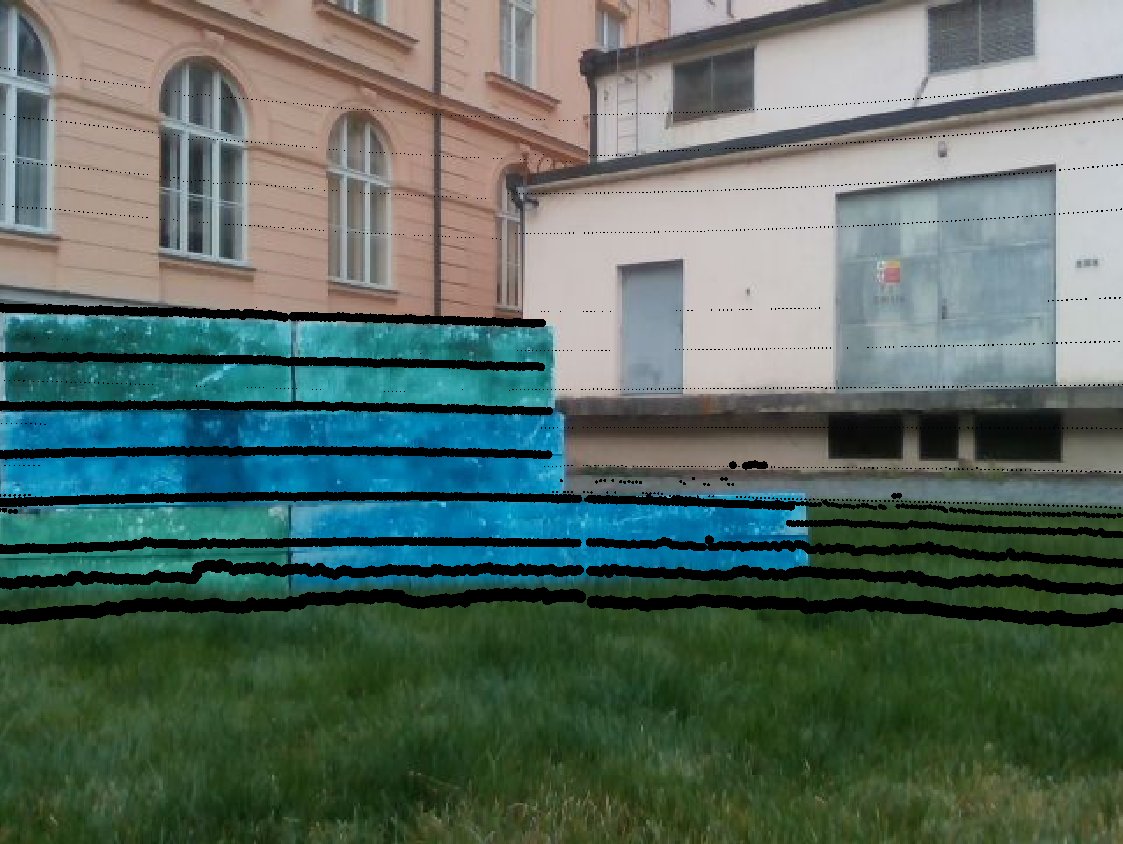
\includegraphics[scale=0.19]{fig/colors_camera}
	\end{subfigure}
	\begin{subfigure}{0.49\textwidth}
		\centering
		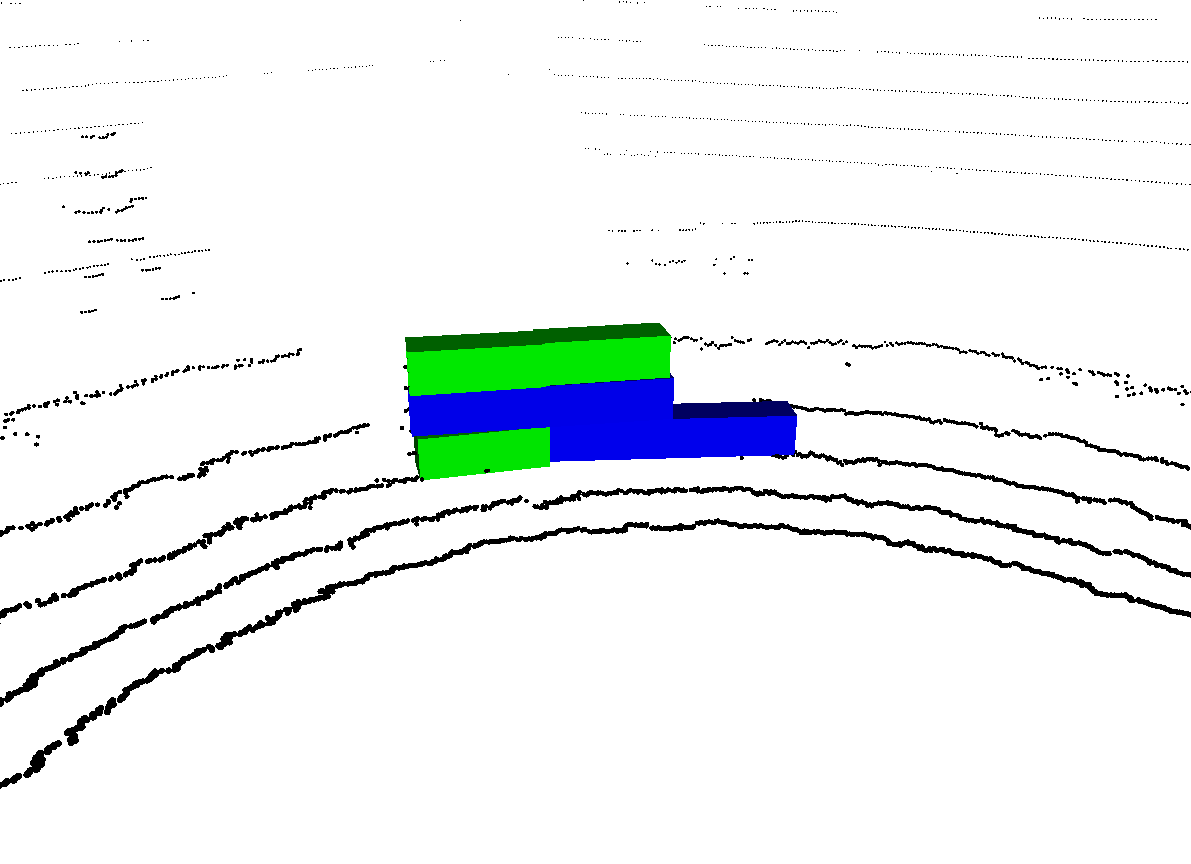
\includegraphics[scale=0.18]{fig/colors_lidar}
	\end{subfigure}
	
	\caption[Colored pointcloud detections]{Detection of bricks using color-based clustering. On the left: Image from a camera pointing at the built wall. Black dots are points captured by the lidar sensor. On the right: Final detection in map frame. All of the bricks are correctly detected, even though they are poorly painted, and the environment is very challenging.}
	\label{fig:colors}
\end{figure}

\newpage

\cleardoublepage

\fancyhead[LO,LE]{EXPERIMENT}
\chapter{Experiment}

The experiment was conducted on the ROS bag taken during the first rehearsal attempt. The robot drove around the perimeter to map the whole arena using the Gmapping package. The brick pattern is placed in the left bottom quadrant and the drone delivery in the right top quadrant of the arena.

 It was surprising that the organizers chose the arena with a significant slope in the middle. We did not expect perfectly flat ground, but the angle of the slope was much higher than our expectations. Besides, the middle part of the arena was made of different - very smooth surface, which negatively influenced odometry, especially in rotation. That makes the localization in the middle much more difficult because, in this place, the robot is tilted, so the laserscan aims into the ground or into the height, and there is also a quite high distance to the nearest significant feature inside the map, which could help to adjust the position. This behavior is visible on the particle cloud during the experiment. When the robot arrives in the middle, the particles are spread into the width. These circumstances caused many problems to teams, which trained for the contest in laboratory grade conditions. Also, it is necessary to mention that there were many people inside the arena during our experiment, which makes the detection even more challenging because people could be easily interpreted as a red pile. Visualization of experiment is shown in the Figure \ref{fig:experiment}.

The robot managed to localize all interest points even though the line segmentation produces a large number of false-positive detections. A significant advantage for the detection is that the clusters are merging measurements from different positions and because the robot is moving during the detections, it is improbable to accumulate multiple false positive detections into the one cluster. Thus these false-positive candidates have very low confidence, and it is not hard for the EM algorithm to find the actual position of interest points.


\begin{figure}[H]
	\centering
	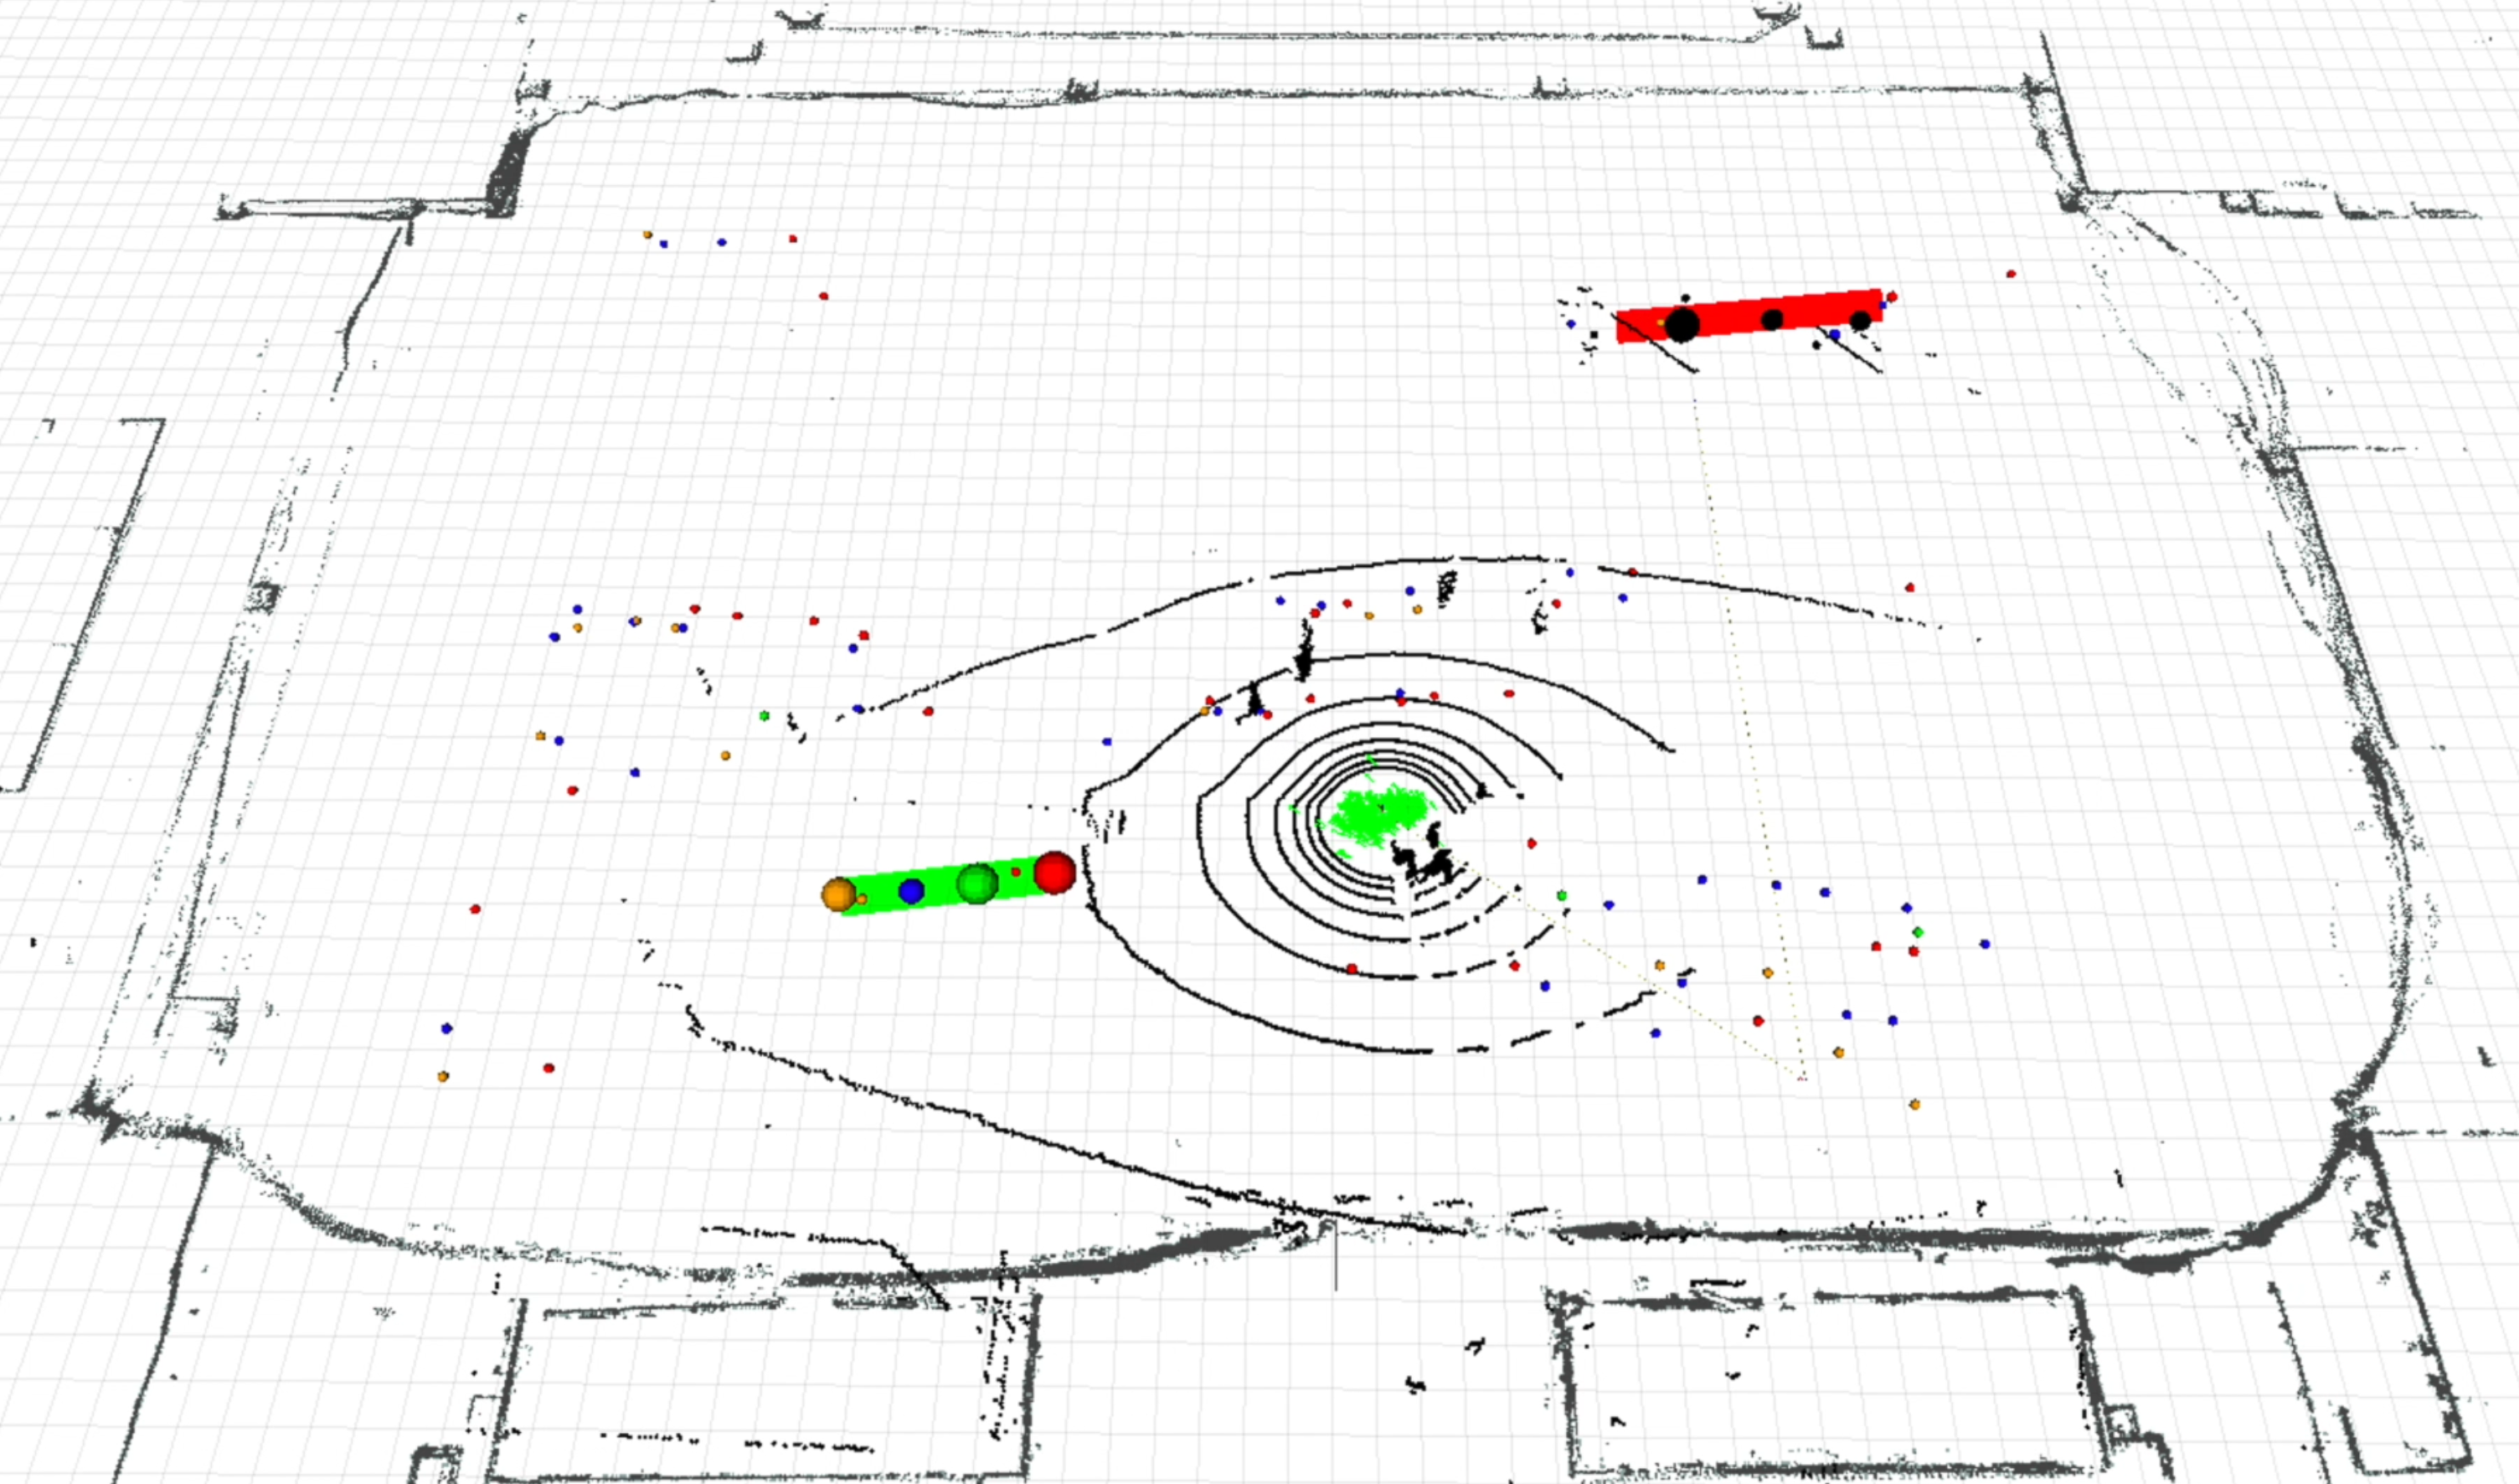
\includegraphics[scale=0.3]{fig/experiment}
	\caption[Experiment results]{In the figure is a screenshot from the experiment. Small spheres on the map are polled clusters from the symbolic map. Different types of detections create these clusters. The size of the sphere represents the confidence of a cluster. The spheres' color corresponds to the color of bricks, and the spheres representing the clusters for UAV destination are colored black. Black is also the pointcloud obtained from lidar and borders of the map. In green color are visualized all particles from the AMCL and also the line representing detection of initial brick pattern. A red line marks the position and rotation of the UAV destination. Note that the RANSAC detector was disabled in this experiment to test the EM algorithm fitting properly. The whole video from the experiment is available at \footnotemark.}
	\label{fig:experiment}
\end{figure}
\footnotetext{\url{https://www.youtube.com/watch?v=KKpCGdJnv7Y} } 

\section{Detector setup}
For experiment was used detection pipeline as desribed in Figure \ref{fig:flowchart}. Value of all constants is listed in Table \ref{tab:constants}.

\begin{table}[H]
	\centering
	\begin{tabular}{cc}
		\toprule
		Constant & Value \\
		\midrule
		$C$ [m] & 0.07   \\ 
		$S$ [m] & 0.07  \\
		$\sigma_x$ [m] & 0.3 \\ 
		$\sigma_y$ [m] & 0.3    \\ 
		$min\_size$ & 10 \\
		$\vec{k}_{pile} $ [m] & [1, 2, 3, 4] \\
		$\vec{k}_{destination}$ [m] & [1, 2, 3, 4] \\
		$d$ [m] & 0.05 \\
		\bottomrule
	\end{tabular}
	\caption{List of constants used in experiment.}
	\label{tab:constants}
\end{table}

\section{Precision of detections}


\newpage
\cleardoublepage

\fancyhead[LO,LE]{CONCLUSION}
\chapter{Conclusion}
\label{ch:conclusion}
The goal of the thesis was to implement a detection algorithm for MBZIRC 2020 contest. More specifically, the algorithm should detect the model of bricks for the second challenge of the contest. The Velodyne VLP-16 lidar sensor was used for the detection. 

A simple line extraction algorithm was applied to find individual bricks. At the beginning of the challenge, the bricks were stacked into the piles, so we applied the EM algorithm to find parameters of individual piles. Further, the piles were always placed with fixed relative positions. Since all the piles together are too large objects for detection in a single measurement, it was necessary to create a global model. In our case, the global model was the symbolic map.

When the robot's localization was used, and all detections were properly transformed and sent to the symbolic map, the initial position of all piles had to be found. We proposed a novel application of the EM algorithm, which can exploit any large object’s spatial distribution. The object was described by a model constructed from the set of normal distributions. Parameters of such a model were found based on partial detections and their confidences. The last type of detection used the RANSAC algorithm to fit individual brick positions to the hypothesis.

There could have been no gap between the bricks when the robot successfully placed them. That made it impossible to distinguish individual bricks by the lidar data. The color camera images were used to color the pointcloud. After coloring, it was possible to use custom clustering and detect individual bricks, that are very close to each other.

In the end, we experimented on the data from the contest, and we have shown that all algorithms work. Although the line extraction algorithm produces a large number of false positives, it is sufficient to detect initial positions of all piles and the UAV destination wall. Different ground segmentation methods were discussed to reduce the number of false-positive measurements. We have also shown that other types of detection have a lower range, but they produce a significantly lower number of false-positive measurements. To sum up, all tasks of the thesis were successfully completed.
\cleardoublepage

\fancyhead[LO,LE]{LIST OF REFERENCES}
% the list of all literature should be supplied in main.bib
\bibliographystyle{unsrt}
\bibliography{main}{}
\clearpage

\appendices
\fancyhead[LO,LE]{APPENDIX}
\section{CD Content}

In Table~\ref{tab:obsah} are listed names of all root directories on CD.

\vspace{1cm}
\begin{table}[!htb]
\centering
\begin{tabular}{lp{10cm}}
\textbf{Directory name} & \textbf{Description} \\

\hline
thesis & the thesis in pdf format \\
ctu\_thesis & latex source codes \\
lidar-gym & OpenAI gym environment \\
\hline
\end{tabular}
\caption{CD Content}
\label{tab:obsah}
\end{table}

\cleardoublepage

\chapter{List of abbreviations}\label{ape:abbreviations}

In Table \ref{table:abbreviations} are listed abbreviations used in this thesis.

\begin{table}[!htb]
\centering
\begin{tabular}{ll}
\textbf{Abbreviation} & \textbf{Meaning} \\
\hline
\textbf{MBZIRC} & Mohamed Bin Zayed International Robotic Challenge \\
\textbf{EM} & Expectation maximization \\
\textbf{RANSAC} & Random sampling consensus \\
\textbf{CNN} & Convolutional neural network \\
\textbf{ROS} & Robot operation system \\
\textbf{lidar} & Light detection and ranging \\
\textbf{MLE} & Maximum likelihood estimate \\
\textbf{UAV} & Unmanned aerial vehicle \\
\textbf{UGV} & Unmanned ground vehicle \\
\textbf{CPU} & Central processing unit\\
\textbf{GPU} & Graphical processing unit \\
\textbf{AMCL} & Adaptive Monte Carlo localization \\
\textbf{IEPF} & Iterative endpoint fit \\
\end{tabular}
\caption{Lists of abbreviations}
\label{table:abbreviations}
\end{table}
\cleardoublepage

\end{document}
